%\documentclass[a4paper]{article}
%\usepackage[italian]{babel}
%\usepackage[utf8]{inputenc}
%\usepackage{amsmath}
%\usepackage{float}
%\usepackage{multirow}
%\usepackage{multicol}
%\usepackage{graphicx}
%\usepackage{siunitx}
%\usepackage{subcaption}
%\usepackage{verbatim}
%\nonstopmode

%\begin{document}
\subsection{Analisi preliminare dei segnali}

Si riportano i dati ottenuti dall'analisi dei segnali dei rivelatori direttamente sull'oscilloscopio. Il segnale
ottenuto è simile per entrambi i rivelatori, sono infatti entrambi negativi e presentano le seguenti caratteristiche:\\

%\begin{minipage} [B]{0.49\linewidth}
%\large{Segnale Rivelatore 1}
%\( T_{salita} \left(10 \% / 90 \% \right) = (4.4 \pm 0.6) ns \) \\
%\( T_{discesa} \left(10 \% / 90 \% \right)= (11.2 \pm 0.6) ns \) \\
%\( Amp = (1.20 \pm 0.03) V  \) \\
%\end{minipage}
%\rule[-1.2cm]{0.3mm}{3cm}
%\begin{minipage} [B]{0.49\linewidth}
%\large{Segnale Rivelatore 2} 
%\( T_{salita} \left(10 \% / 90 \% \right)= (3.8 \pm 0.3) ns \) \\
%\( T_{discesa} \left(10 \% / 90 \% \right)= (10.8 \pm 0.6) ns \) \\
%\( Amp = (1.16 \pm 0.03) V  \) \\
%\end{minipage}
%\vspace{0.5 cm}
%
\begin{tabella}[h]
	\centering
	\begin{center}
\begin{tabulary}{\textwidth}{CCCCCCC}
\toprule
Rivelatore	& Ampiezza  [V]	& Errore [V]	& Tempo salita [ns]	& Errore [ns]	& Tempo discesa [ns]	& Errore [ns]	\\ \midrule
1		& 1.20		& 0.03		& 4.4			& 0.6		& 11.2			& 0.6		\\ \midrule
2		& 1.16		& 0.03		& 3.8			& 0.3		& 10.8			& 0.6		\\
\bottomrule
\end{tabulary}
\end{center}

	\caption{Le misure preliminari in uscita dei rivelatori}
	\label{tab:calib_pre}
\end{tabella}
%

Per misurare i tempi di salita (allontanamento dalla baseline) e di discesa si è misurato il tempo impiegato dal segnale per passare dal 10\% al 90\% dell'ampiezza
massima per la discesa e viceversa per la salita; gli errori sono stati stimati come semplici errori associati alla lettura da oscilloscopio.\\

%A questo punto si è voluto visualizzare  il segnale bipolare dell'amplificatore ORTEC 855, costituito a sua volta da una moltitudine di segnali di ampiezza variabile, proporzionali
%all'energia rilasciata dai fotoni nel rivelatore. I segnali di ampiezza massima (non prendendo in considerazione segnali totalmente fuori scala imputabili ad esempio ad eventuali
%raggi cosmici) sono quelli corrispondenti al Compton Edge del fotone a 1275 KeV. Triggherando con il segnale logico del CFTD di un rivelatore ed osservando l'output bipolare dell'altro,
%si è invece in grado di vedere gli eventi in coincidenza (fotoni emessi back to back) e di conseguenza i segnali ad ampiezza massima corrispondono al Compton Edge del fotone a 511KeV.

\subsection{Calibrazione in Energia}
Gli spettri presi presentano i classici Compton edge relativi ai fotoni a 511KeV e 1275KeV riconducibili rispettivamente
all'annichilazione del positrone prodotto dal decadimento della sorgente di sodio ed un elettrone presente nel materiale ed il decadimento gamma del neon. Le due spalle Compton possono
essere interpolate tramite una gaussiana di cui ci si ricava centroide e sigma. I centroidi non corrispondono però con i Compton edge veri e propri, che valgono
340KeV e 1062KeV per i due fotoni sopracitati: infatti al crescere della sigma si osserva uno shift verso sinistra dei centroidi relativi alle due spalle Compton
per effetto della risoluzione finita dello strumento. \\
Si può però correlare il parametro adimensionale \(\frac{s}{C}\) con il valore in KeV della sigma e quest'ultima al valore dello shift tramite delle funzioni di 
risposta, in maniera tale da poter associare al centroide un valore in energia pari a \(E_{\text{centroide}} = E_{\text{CE}} - E_{\text{shift}}\).  Nelle tabelle
sottostanti si possono leggere i parametri ottenuti interpolando i Compton edge e le conseguenti correzioni del valore in energia dei centroidi\footnote{I grafici
delle interpolazioni si possono vedere nelle \textit{appendici}.}. Poichè questa procedura è stata effettuata a mano non è stato possibile fare una stima degli errori 
associati alle energie dei Compton edge.


%
\begin{tabella}[h]
	\centering
	\begin{center}
\begin{tabulary}{\textwidth}{CCCCCC}
\toprule
Centroide	& s	& s/C		& $\sigma$ [KeV]	& Shift [KeV]	& Centroide [KeV]	\\ \midrule
239.7		& 48.4	& 0.202		& 38			& 57		& 283			\\ \midrule
801.9		& 78.0	& 0.0972	& 77			& 132 		& 930			\\
\bottomrule
\end{tabulary}
\end{center}


	\caption{Procedura calibrazione del rivelatore 1}
	\label{tab:calib_shift_1}
\end{tabella}
%
%
\begin{tabella}[h]
	\centering
	\begin{center}
\begin{tabulary}{\textwidth}{CCCCCC}
\toprule
Centroide	& s	& s/C		& $\sigma$ [KeV]	& Shift [KeV]	& Centroide [KeV]	\\ \midrule
297.1		& 60.4	& 0.203		& 38			& 57		& 283			\\ \midrule
930  		& 92.7	& 0.0951	& 78			& 132 		& 930			\\
\bottomrule
\end{tabulary}
\end{center}


	\caption{Procedura calibrazione del rivelatore 2}
	\label{tab:calib__shift_2}
\end{tabella}
%
Avendo quindi due coppie di valori corrispondeti ai due Compton edge, è possibile ottenere un grafico che permette di calibrare gli spettri in energia.
Essendo i punti a disposizione per ogniuna delle interpolazioni solamente due non si è potuto fornire gli errori relativi ai parametri dell'interpolazione. Inoltre per
trovare i centroidi è stata eseguita la correzione dovuta alla finitezza della risoluzione sopra descritta; dato che questa correzione fa uso di grafici ottenuti
sperimentalmente senza errori, non si è ritenuto opportuna la stima di errori legati ai parametri di calibrazione.


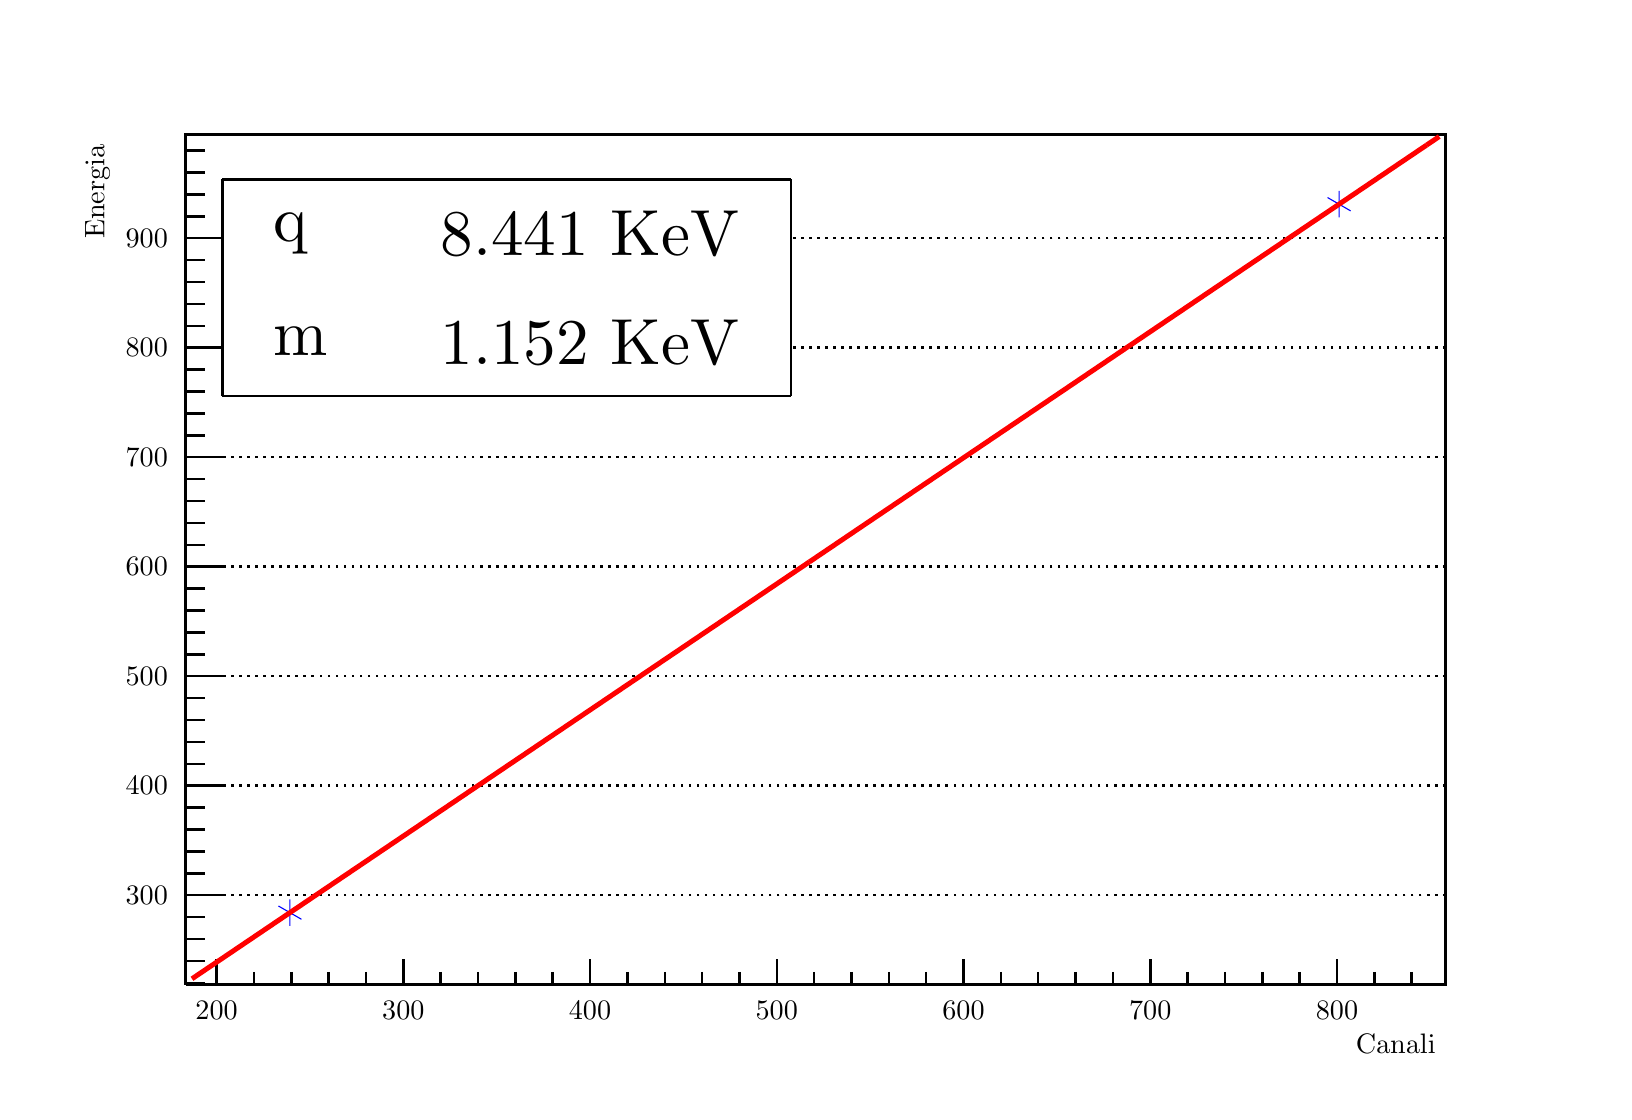
\begin{tikzpicture}
\pgfdeclareplotmark{cross} {
\pgfpathmoveto{\pgfpoint{-0.3\pgfplotmarksize}{\pgfplotmarksize}}
\pgfpathlineto{\pgfpoint{+0.3\pgfplotmarksize}{\pgfplotmarksize}}
\pgfpathlineto{\pgfpoint{+0.3\pgfplotmarksize}{0.3\pgfplotmarksize}}
\pgfpathlineto{\pgfpoint{+1\pgfplotmarksize}{0.3\pgfplotmarksize}}
\pgfpathlineto{\pgfpoint{+1\pgfplotmarksize}{-0.3\pgfplotmarksize}}
\pgfpathlineto{\pgfpoint{+0.3\pgfplotmarksize}{-0.3\pgfplotmarksize}}
\pgfpathlineto{\pgfpoint{+0.3\pgfplotmarksize}{-1.\pgfplotmarksize}}
\pgfpathlineto{\pgfpoint{-0.3\pgfplotmarksize}{-1.\pgfplotmarksize}}
\pgfpathlineto{\pgfpoint{-0.3\pgfplotmarksize}{-0.3\pgfplotmarksize}}
\pgfpathlineto{\pgfpoint{-1.\pgfplotmarksize}{-0.3\pgfplotmarksize}}
\pgfpathlineto{\pgfpoint{-1.\pgfplotmarksize}{0.3\pgfplotmarksize}}
\pgfpathlineto{\pgfpoint{-0.3\pgfplotmarksize}{0.3\pgfplotmarksize}}
\pgfpathclose
\pgfusepathqstroke
}
\pgfdeclareplotmark{cross*} {
\pgfpathmoveto{\pgfpoint{-0.3\pgfplotmarksize}{\pgfplotmarksize}}
\pgfpathlineto{\pgfpoint{+0.3\pgfplotmarksize}{\pgfplotmarksize}}
\pgfpathlineto{\pgfpoint{+0.3\pgfplotmarksize}{0.3\pgfplotmarksize}}
\pgfpathlineto{\pgfpoint{+1\pgfplotmarksize}{0.3\pgfplotmarksize}}
\pgfpathlineto{\pgfpoint{+1\pgfplotmarksize}{-0.3\pgfplotmarksize}}
\pgfpathlineto{\pgfpoint{+0.3\pgfplotmarksize}{-0.3\pgfplotmarksize}}
\pgfpathlineto{\pgfpoint{+0.3\pgfplotmarksize}{-1.\pgfplotmarksize}}
\pgfpathlineto{\pgfpoint{-0.3\pgfplotmarksize}{-1.\pgfplotmarksize}}
\pgfpathlineto{\pgfpoint{-0.3\pgfplotmarksize}{-0.3\pgfplotmarksize}}
\pgfpathlineto{\pgfpoint{-1.\pgfplotmarksize}{-0.3\pgfplotmarksize}}
\pgfpathlineto{\pgfpoint{-1.\pgfplotmarksize}{0.3\pgfplotmarksize}}
\pgfpathlineto{\pgfpoint{-0.3\pgfplotmarksize}{0.3\pgfplotmarksize}}
\pgfpathclose
\pgfusepathqfillstroke
}
\pgfdeclareplotmark{newstar} {
\pgfpathmoveto{\pgfqpoint{0pt}{\pgfplotmarksize}}
\pgfpathlineto{\pgfqpointpolar{44}{0.5\pgfplotmarksize}}
\pgfpathlineto{\pgfqpointpolar{18}{\pgfplotmarksize}}
\pgfpathlineto{\pgfqpointpolar{-20}{0.5\pgfplotmarksize}}
\pgfpathlineto{\pgfqpointpolar{-54}{\pgfplotmarksize}}
\pgfpathlineto{\pgfqpointpolar{-90}{0.5\pgfplotmarksize}}
\pgfpathlineto{\pgfqpointpolar{234}{\pgfplotmarksize}}
\pgfpathlineto{\pgfqpointpolar{198}{0.5\pgfplotmarksize}}
\pgfpathlineto{\pgfqpointpolar{162}{\pgfplotmarksize}}
\pgfpathlineto{\pgfqpointpolar{134}{0.5\pgfplotmarksize}}
\pgfpathclose
\pgfusepathqstroke
}
\pgfdeclareplotmark{newstar*} {
\pgfpathmoveto{\pgfqpoint{0pt}{\pgfplotmarksize}}
\pgfpathlineto{\pgfqpointpolar{44}{0.5\pgfplotmarksize}}
\pgfpathlineto{\pgfqpointpolar{18}{\pgfplotmarksize}}
\pgfpathlineto{\pgfqpointpolar{-20}{0.5\pgfplotmarksize}}
\pgfpathlineto{\pgfqpointpolar{-54}{\pgfplotmarksize}}
\pgfpathlineto{\pgfqpointpolar{-90}{0.5\pgfplotmarksize}}
\pgfpathlineto{\pgfqpointpolar{234}{\pgfplotmarksize}}
\pgfpathlineto{\pgfqpointpolar{198}{0.5\pgfplotmarksize}}
\pgfpathlineto{\pgfqpointpolar{162}{\pgfplotmarksize}}
\pgfpathlineto{\pgfqpointpolar{134}{0.5\pgfplotmarksize}}
\pgfpathclose
\pgfusepathqfillstroke
}
\definecolor{c}{rgb}{1,1,1};
\draw [color=c, fill=c] (0,0) rectangle (20,13.4957);
\draw [color=c, fill=c] (2,1.34957) rectangle (18,12.1461);
\definecolor{c}{rgb}{0,0,0};
\draw [c,line width=0.9] (2,1.34957) -- (2,12.1461) -- (18,12.1461) -- (18,1.34957) -- (2,1.34957);
\definecolor{c}{rgb}{1,1,1};
\draw [color=c, fill=c] (2,1.34957) rectangle (18,12.1461);
\definecolor{c}{rgb}{0,0,0};
\draw [c,line width=0.9] (2,1.34957) -- (2,12.1461) -- (18,12.1461) -- (18,1.34957) -- (2,1.34957);
\draw [c,line width=0.9] (2,1.34957) -- (18,1.34957);
\draw [c,line width=0.9] (2,1.34957) -- (2,12.1461);
\draw [c,dotted,line width=0.9] (18,2.48568) -- (2,2.48568);
\draw [c,dotted,line width=0.9] (18,3.87628) -- (2,3.87628);
\draw [c,dotted,line width=0.9] (18,5.26687) -- (2,5.26687);
\draw [c,dotted,line width=0.9] (18,6.65746) -- (2,6.65746);
\draw [c,dotted,line width=0.9] (18,8.04805) -- (2,8.04805);
\draw [c,dotted,line width=0.9] (18,9.43865) -- (2,9.43865);
\draw [c,dotted,line width=0.9] (18,10.8292) -- (2,10.8292);
\draw [c,dotted,line width=0.9] (18,2.48568) -- (2,2.48568);
\draw [c,dotted,line width=0.9] (18,10.8292) -- (2,10.8292);
\draw [c,line width=0.9] (2,1.34957) -- (18,1.34957);
\draw [anchor= east] (18,0.593811) node[scale=1.01821, color=c, rotate=0]{Canali};
\draw [c,line width=0.9] (2.39179,1.67347) -- (2.39179,1.34957);
\draw [c,line width=0.9] (2.86612,1.51152) -- (2.86612,1.34957);
\draw [c,line width=0.9] (3.34045,1.51152) -- (3.34045,1.34957);
\draw [c,line width=0.9] (3.81478,1.51152) -- (3.81478,1.34957);
\draw [c,line width=0.9] (4.2891,1.51152) -- (4.2891,1.34957);
\draw [c,line width=0.9] (4.76343,1.67347) -- (4.76343,1.34957);
\draw [c,line width=0.9] (5.23776,1.51152) -- (5.23776,1.34957);
\draw [c,line width=0.9] (5.71208,1.51152) -- (5.71208,1.34957);
\draw [c,line width=0.9] (6.18641,1.51152) -- (6.18641,1.34957);
\draw [c,line width=0.9] (6.66074,1.51152) -- (6.66074,1.34957);
\draw [c,line width=0.9] (7.13506,1.67347) -- (7.13506,1.34957);
\draw [c,line width=0.9] (7.60939,1.51152) -- (7.60939,1.34957);
\draw [c,line width=0.9] (8.08372,1.51152) -- (8.08372,1.34957);
\draw [c,line width=0.9] (8.55805,1.51152) -- (8.55805,1.34957);
\draw [c,line width=0.9] (9.03237,1.51152) -- (9.03237,1.34957);
\draw [c,line width=0.9] (9.5067,1.67347) -- (9.5067,1.34957);
\draw [c,line width=0.9] (9.98103,1.51152) -- (9.98103,1.34957);
\draw [c,line width=0.9] (10.4554,1.51152) -- (10.4554,1.34957);
\draw [c,line width=0.9] (10.9297,1.51152) -- (10.9297,1.34957);
\draw [c,line width=0.9] (11.404,1.51152) -- (11.404,1.34957);
\draw [c,line width=0.9] (11.8783,1.67347) -- (11.8783,1.34957);
\draw [c,line width=0.9] (12.3527,1.51152) -- (12.3527,1.34957);
\draw [c,line width=0.9] (12.827,1.51152) -- (12.827,1.34957);
\draw [c,line width=0.9] (13.3013,1.51152) -- (13.3013,1.34957);
\draw [c,line width=0.9] (13.7756,1.51152) -- (13.7756,1.34957);
\draw [c,line width=0.9] (14.25,1.67347) -- (14.25,1.34957);
\draw [c,line width=0.9] (14.7243,1.51152) -- (14.7243,1.34957);
\draw [c,line width=0.9] (15.1986,1.51152) -- (15.1986,1.34957);
\draw [c,line width=0.9] (15.673,1.51152) -- (15.673,1.34957);
\draw [c,line width=0.9] (16.1473,1.51152) -- (16.1473,1.34957);
\draw [c,line width=0.9] (16.6216,1.67347) -- (16.6216,1.34957);
\draw [c,line width=0.9] (2.39179,1.67347) -- (2.39179,1.34957);
\draw [c,line width=0.9] (16.6216,1.67347) -- (16.6216,1.34957);
\draw [c,line width=0.9] (17.0959,1.51152) -- (17.0959,1.34957);
\draw [c,line width=0.9] (17.5703,1.51152) -- (17.5703,1.34957);
\draw [anchor=base] (2.39179,0.904212) node[scale=1.01821, color=c, rotate=0]{200};
\draw [anchor=base] (4.76343,0.904212) node[scale=1.01821, color=c, rotate=0]{300};
\draw [anchor=base] (7.13506,0.904212) node[scale=1.01821, color=c, rotate=0]{400};
\draw [anchor=base] (9.5067,0.904212) node[scale=1.01821, color=c, rotate=0]{500};
\draw [anchor=base] (11.8783,0.904212) node[scale=1.01821, color=c, rotate=0]{600};
\draw [anchor=base] (14.25,0.904212) node[scale=1.01821, color=c, rotate=0]{700};
\draw [anchor=base] (16.6216,0.904212) node[scale=1.01821, color=c, rotate=0]{800};
\draw [c,line width=0.9] (2,1.34957) -- (2,12.1461);
\draw [anchor= east] (0.88,12.1461) node[scale=1.01821, color=c, rotate=90]{Energia};
\draw [c,line width=0.9] (2.48,2.48568) -- (2,2.48568);
\draw [c,line width=0.9] (2.24,2.7638) -- (2,2.7638);
\draw [c,line width=0.9] (2.24,3.04192) -- (2,3.04192);
\draw [c,line width=0.9] (2.24,3.32004) -- (2,3.32004);
\draw [c,line width=0.9] (2.24,3.59816) -- (2,3.59816);
\draw [c,line width=0.9] (2.48,3.87628) -- (2,3.87628);
\draw [c,line width=0.9] (2.24,4.1544) -- (2,4.1544);
\draw [c,line width=0.9] (2.24,4.43251) -- (2,4.43251);
\draw [c,line width=0.9] (2.24,4.71063) -- (2,4.71063);
\draw [c,line width=0.9] (2.24,4.98875) -- (2,4.98875);
\draw [c,line width=0.9] (2.48,5.26687) -- (2,5.26687);
\draw [c,line width=0.9] (2.24,5.54499) -- (2,5.54499);
\draw [c,line width=0.9] (2.24,5.82311) -- (2,5.82311);
\draw [c,line width=0.9] (2.24,6.10123) -- (2,6.10123);
\draw [c,line width=0.9] (2.24,6.37934) -- (2,6.37934);
\draw [c,line width=0.9] (2.48,6.65746) -- (2,6.65746);
\draw [c,line width=0.9] (2.24,6.93558) -- (2,6.93558);
\draw [c,line width=0.9] (2.24,7.2137) -- (2,7.2137);
\draw [c,line width=0.9] (2.24,7.49182) -- (2,7.49182);
\draw [c,line width=0.9] (2.24,7.76994) -- (2,7.76994);
\draw [c,line width=0.9] (2.48,8.04805) -- (2,8.04805);
\draw [c,line width=0.9] (2.24,8.32617) -- (2,8.32617);
\draw [c,line width=0.9] (2.24,8.60429) -- (2,8.60429);
\draw [c,line width=0.9] (2.24,8.88241) -- (2,8.88241);
\draw [c,line width=0.9] (2.24,9.16053) -- (2,9.16053);
\draw [c,line width=0.9] (2.48,9.43865) -- (2,9.43865);
\draw [c,line width=0.9] (2.24,9.71677) -- (2,9.71677);
\draw [c,line width=0.9] (2.24,9.99488) -- (2,9.99488);
\draw [c,line width=0.9] (2.24,10.273) -- (2,10.273);
\draw [c,line width=0.9] (2.24,10.5511) -- (2,10.5511);
\draw [c,line width=0.9] (2.48,10.8292) -- (2,10.8292);
\draw [c,line width=0.9] (2.48,2.48568) -- (2,2.48568);
\draw [c,line width=0.9] (2.24,2.20757) -- (2,2.20757);
\draw [c,line width=0.9] (2.24,1.92945) -- (2,1.92945);
\draw [c,line width=0.9] (2.24,1.65133) -- (2,1.65133);
\draw [c,line width=0.9] (2.24,1.37321) -- (2,1.37321);
\draw [c,line width=0.9] (2.48,10.8292) -- (2,10.8292);
\draw [c,line width=0.9] (2.24,11.1074) -- (2,11.1074);
\draw [c,line width=0.9] (2.24,11.3855) -- (2,11.3855);
\draw [c,line width=0.9] (2.24,11.6636) -- (2,11.6636);
\draw [c,line width=0.9] (2.24,11.9417) -- (2,11.9417);
\draw [anchor= east] (1.9,2.48568) node[scale=1.01821, color=c, rotate=0]{300};
\draw [anchor= east] (1.9,3.87628) node[scale=1.01821, color=c, rotate=0]{400};
\draw [anchor= east] (1.9,5.26687) node[scale=1.01821, color=c, rotate=0]{500};
\draw [anchor= east] (1.9,6.65746) node[scale=1.01821, color=c, rotate=0]{600};
\draw [anchor= east] (1.9,8.04805) node[scale=1.01821, color=c, rotate=0]{700};
\draw [anchor= east] (1.9,9.43865) node[scale=1.01821, color=c, rotate=0]{800};
\draw [anchor= east] (1.9,10.8292) node[scale=1.01821, color=c, rotate=0]{900};
\definecolor{c}{rgb}{1,1,1};
\draw [color=c, fill=c] (2.46418,8.82521) rectangle (9.68481,11.5759);
\definecolor{c}{rgb}{0,0,0};
\draw [c,line width=0.9] (2.46418,8.82521) -- (9.68481,8.82521);
\draw [c,line width=0.9] (9.68481,8.82521) -- (9.68481,11.5759);
\draw [c,line width=0.9] (9.68481,11.5759) -- (2.46418,11.5759);
\draw [c,line width=0.9] (2.46418,11.5759) -- (2.46418,8.82521);
\draw [anchor= west] (2.82521,10.8883) node[scale=1.3364, color=c, rotate=0]{q       };
\draw [anchor= east] (9.32378,10.8883) node[scale=1.3364, color=c, rotate=0]{$ 8.441$ KeV};
\draw [anchor= west] (2.82521,9.51289) node[scale=1.3364, color=c, rotate=0]{m       };
\draw [anchor= east] (9.32378,9.51289) node[scale=1.3364, color=c, rotate=0]{$ 1.152$ KeV};
\definecolor{c}{rgb}{0,0,1};
\foreach \P in {(3.32378,2.26361),(16.6476,11.2607)}{\draw[mark options={color=c,fill=c},mark size=4.804805pt,mark=asterisk] plot coordinates {\P};}
\definecolor{c}{rgb}{1,0,0};
\draw [c,line width=1.8] (2.08,1.42372) -- (2.24,1.53177) -- (2.4,1.63981) -- (2.56,1.74785) -- (2.72,1.8559) -- (2.88,1.96394) -- (3.04,2.07198) -- (3.2,2.18002) -- (3.36,2.28807) -- (3.52,2.39611) -- (3.68,2.50415) -- (3.84,2.6122) -- (4,2.72024)
 -- (4.16,2.82828) -- (4.32,2.93633) -- (4.48,3.04437) -- (4.64,3.15241) -- (4.8,3.26045) -- (4.96,3.3685) -- (5.12,3.47654) -- (5.28,3.58458) -- (5.44,3.69263) -- (5.6,3.80067) -- (5.76,3.90871) -- (5.92,4.01676) -- (6.08,4.1248) -- (6.24,4.23284)
 -- (6.4,4.34088) -- (6.56,4.44893) -- (6.72,4.55697) -- (6.88,4.66501) -- (7.04,4.77306) -- (7.2,4.8811) -- (7.36,4.98914) -- (7.52,5.09719) -- (7.68,5.20523) -- (7.84,5.31327) -- (8,5.42131) -- (8.16,5.52936) -- (8.32,5.6374) -- (8.48,5.74544) --
 (8.64,5.85349) -- (8.8,5.96153) -- (8.96,6.06957) -- (9.12,6.17762) -- (9.28,6.28566) -- (9.44,6.3937) -- (9.6,6.50174) -- (9.76,6.60979) -- (9.92,6.71783);
\draw [c,line width=1.8] (9.92,6.71783) -- (10.08,6.82587) -- (10.24,6.93392) -- (10.4,7.04196) -- (10.56,7.15) -- (10.72,7.25805) -- (10.88,7.36609) -- (11.04,7.47413) -- (11.2,7.58217) -- (11.36,7.69022) -- (11.52,7.79826) -- (11.68,7.9063) --
 (11.84,8.01435) -- (12,8.12239) -- (12.16,8.23043) -- (12.32,8.33848) -- (12.48,8.44652) -- (12.64,8.55456) -- (12.8,8.6626) -- (12.96,8.77065) -- (13.12,8.87869) -- (13.28,8.98673) -- (13.44,9.09478) -- (13.6,9.20282) -- (13.76,9.31086) --
 (13.92,9.41891) -- (14.08,9.52695) -- (14.24,9.63499) -- (14.4,9.74303) -- (14.56,9.85108) -- (14.72,9.95912) -- (14.88,10.0672) -- (15.04,10.1752) -- (15.2,10.2832) -- (15.36,10.3913) -- (15.52,10.4993) -- (15.68,10.6074) -- (15.84,10.7154) --
 (16,10.8235) -- (16.16,10.9315) -- (16.32,11.0396) -- (16.48,11.1476) -- (16.64,11.2556) -- (16.8,11.3637) -- (16.96,11.4717) -- (17.12,11.5798) -- (17.28,11.6878) -- (17.44,11.7959) -- (17.6,11.9039) -- (17.76,12.0119);
\draw [c,line width=1.8] (17.76,12.0119) -- (17.92,12.12);
\definecolor{c}{rgb}{1,1,1};
\draw [color=c, fill=c] (2.46418,8.82521) rectangle (9.68481,11.5759);
\definecolor{c}{rgb}{0,0,0};
\draw [c,line width=0.9] (2.46418,8.82521) -- (9.68481,8.82521);
\draw [c,line width=0.9] (9.68481,8.82521) -- (9.68481,11.5759);
\draw [c,line width=0.9] (9.68481,11.5759) -- (2.46418,11.5759);
\draw [c,line width=0.9] (2.46418,11.5759) -- (2.46418,8.82521);
\draw [anchor= west] (2.82521,10.8883) node[scale=2.35461, color=c, rotate=0]{q       };
\draw [anchor= east] (9.32378,10.8883) node[scale=2.35461, color=c, rotate=0]{$ 8.441$ KeV};
\draw [anchor= west] (2.82521,9.51289) node[scale=2.35461, color=c, rotate=0]{m       };
\draw [anchor= east] (9.32378,9.51289) node[scale=2.35461, color=c, rotate=0]{$ 1.152$ KeV};
%\draw (10,12.808) node[scale=1.40004, color=c, rotate=0]{Calibrazione Energia Rivelatore 1};
\end{tikzpicture}

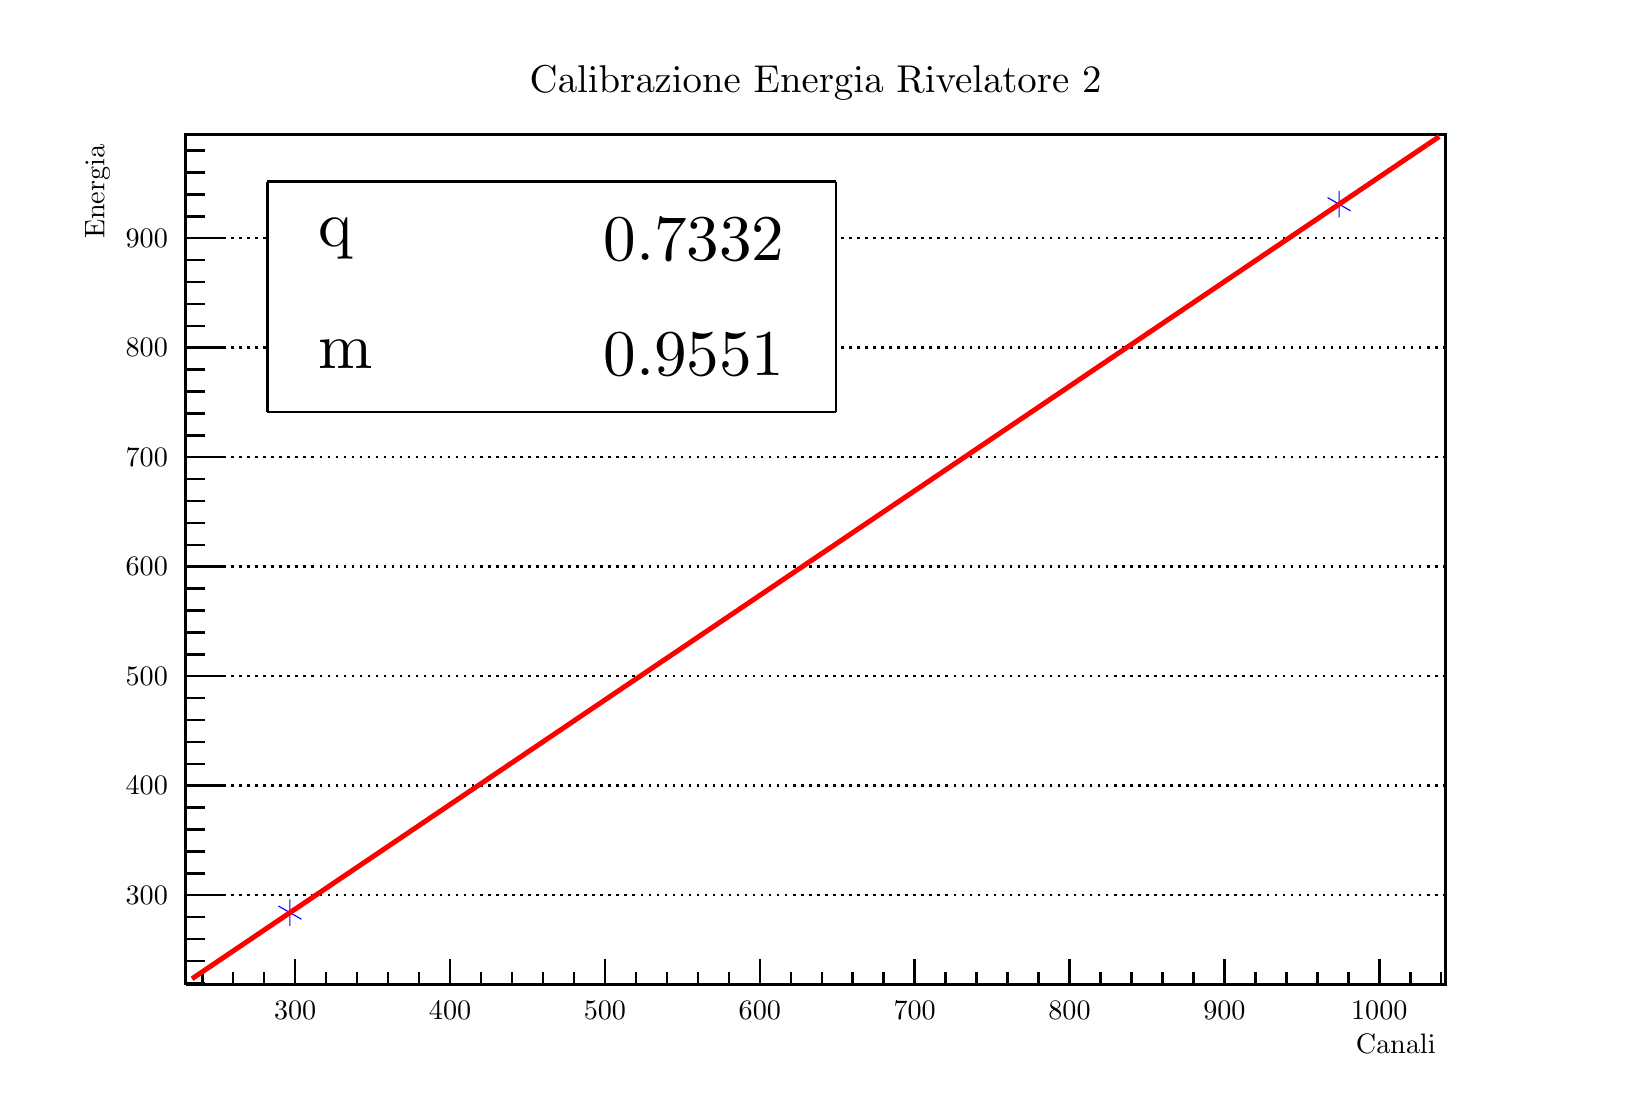
\begin{tikzpicture}
\pgfdeclareplotmark{cross} {
\pgfpathmoveto{\pgfpoint{-0.3\pgfplotmarksize}{\pgfplotmarksize}}
\pgfpathlineto{\pgfpoint{+0.3\pgfplotmarksize}{\pgfplotmarksize}}
\pgfpathlineto{\pgfpoint{+0.3\pgfplotmarksize}{0.3\pgfplotmarksize}}
\pgfpathlineto{\pgfpoint{+1\pgfplotmarksize}{0.3\pgfplotmarksize}}
\pgfpathlineto{\pgfpoint{+1\pgfplotmarksize}{-0.3\pgfplotmarksize}}
\pgfpathlineto{\pgfpoint{+0.3\pgfplotmarksize}{-0.3\pgfplotmarksize}}
\pgfpathlineto{\pgfpoint{+0.3\pgfplotmarksize}{-1.\pgfplotmarksize}}
\pgfpathlineto{\pgfpoint{-0.3\pgfplotmarksize}{-1.\pgfplotmarksize}}
\pgfpathlineto{\pgfpoint{-0.3\pgfplotmarksize}{-0.3\pgfplotmarksize}}
\pgfpathlineto{\pgfpoint{-1.\pgfplotmarksize}{-0.3\pgfplotmarksize}}
\pgfpathlineto{\pgfpoint{-1.\pgfplotmarksize}{0.3\pgfplotmarksize}}
\pgfpathlineto{\pgfpoint{-0.3\pgfplotmarksize}{0.3\pgfplotmarksize}}
\pgfpathclose
\pgfusepathqstroke
}
\pgfdeclareplotmark{cross*} {
\pgfpathmoveto{\pgfpoint{-0.3\pgfplotmarksize}{\pgfplotmarksize}}
\pgfpathlineto{\pgfpoint{+0.3\pgfplotmarksize}{\pgfplotmarksize}}
\pgfpathlineto{\pgfpoint{+0.3\pgfplotmarksize}{0.3\pgfplotmarksize}}
\pgfpathlineto{\pgfpoint{+1\pgfplotmarksize}{0.3\pgfplotmarksize}}
\pgfpathlineto{\pgfpoint{+1\pgfplotmarksize}{-0.3\pgfplotmarksize}}
\pgfpathlineto{\pgfpoint{+0.3\pgfplotmarksize}{-0.3\pgfplotmarksize}}
\pgfpathlineto{\pgfpoint{+0.3\pgfplotmarksize}{-1.\pgfplotmarksize}}
\pgfpathlineto{\pgfpoint{-0.3\pgfplotmarksize}{-1.\pgfplotmarksize}}
\pgfpathlineto{\pgfpoint{-0.3\pgfplotmarksize}{-0.3\pgfplotmarksize}}
\pgfpathlineto{\pgfpoint{-1.\pgfplotmarksize}{-0.3\pgfplotmarksize}}
\pgfpathlineto{\pgfpoint{-1.\pgfplotmarksize}{0.3\pgfplotmarksize}}
\pgfpathlineto{\pgfpoint{-0.3\pgfplotmarksize}{0.3\pgfplotmarksize}}
\pgfpathclose
\pgfusepathqfillstroke
}
\pgfdeclareplotmark{newstar} {
\pgfpathmoveto{\pgfqpoint{0pt}{\pgfplotmarksize}}
\pgfpathlineto{\pgfqpointpolar{44}{0.5\pgfplotmarksize}}
\pgfpathlineto{\pgfqpointpolar{18}{\pgfplotmarksize}}
\pgfpathlineto{\pgfqpointpolar{-20}{0.5\pgfplotmarksize}}
\pgfpathlineto{\pgfqpointpolar{-54}{\pgfplotmarksize}}
\pgfpathlineto{\pgfqpointpolar{-90}{0.5\pgfplotmarksize}}
\pgfpathlineto{\pgfqpointpolar{234}{\pgfplotmarksize}}
\pgfpathlineto{\pgfqpointpolar{198}{0.5\pgfplotmarksize}}
\pgfpathlineto{\pgfqpointpolar{162}{\pgfplotmarksize}}
\pgfpathlineto{\pgfqpointpolar{134}{0.5\pgfplotmarksize}}
\pgfpathclose
\pgfusepathqstroke
}
\pgfdeclareplotmark{newstar*} {
\pgfpathmoveto{\pgfqpoint{0pt}{\pgfplotmarksize}}
\pgfpathlineto{\pgfqpointpolar{44}{0.5\pgfplotmarksize}}
\pgfpathlineto{\pgfqpointpolar{18}{\pgfplotmarksize}}
\pgfpathlineto{\pgfqpointpolar{-20}{0.5\pgfplotmarksize}}
\pgfpathlineto{\pgfqpointpolar{-54}{\pgfplotmarksize}}
\pgfpathlineto{\pgfqpointpolar{-90}{0.5\pgfplotmarksize}}
\pgfpathlineto{\pgfqpointpolar{234}{\pgfplotmarksize}}
\pgfpathlineto{\pgfqpointpolar{198}{0.5\pgfplotmarksize}}
\pgfpathlineto{\pgfqpointpolar{162}{\pgfplotmarksize}}
\pgfpathlineto{\pgfqpointpolar{134}{0.5\pgfplotmarksize}}
\pgfpathclose
\pgfusepathqfillstroke
}
\definecolor{c}{rgb}{1,1,1};
\draw [color=c, fill=c] (0,0) rectangle (20,13.4957);
\draw [color=c, fill=c] (2,1.34957) rectangle (18,12.1461);
\definecolor{c}{rgb}{0,0,0};
\draw [c,line width=0.9] (2,1.34957) -- (2,12.1461) -- (18,12.1461) -- (18,1.34957) -- (2,1.34957);
\definecolor{c}{rgb}{1,1,1};
\draw [color=c, fill=c] (2,1.34957) rectangle (18,12.1461);
\definecolor{c}{rgb}{0,0,0};
\draw [c,line width=0.9] (2,1.34957) -- (2,12.1461) -- (18,12.1461) -- (18,1.34957) -- (2,1.34957);
\draw [c,line width=0.9] (2,1.34957) -- (18,1.34957);
\draw [c,line width=0.9] (2,1.34957) -- (2,12.1461);
\draw [c,dotted,line width=0.9] (18,2.48568) -- (2,2.48568);
\draw [c,dotted,line width=0.9] (18,3.87628) -- (2,3.87628);
\draw [c,dotted,line width=0.9] (18,5.26687) -- (2,5.26687);
\draw [c,dotted,line width=0.9] (18,6.65746) -- (2,6.65746);
\draw [c,dotted,line width=0.9] (18,8.04805) -- (2,8.04805);
\draw [c,dotted,line width=0.9] (18,9.43865) -- (2,9.43865);
\draw [c,dotted,line width=0.9] (18,10.8292) -- (2,10.8292);
\draw [c,dotted,line width=0.9] (18,2.48568) -- (2,2.48568);
\draw [c,dotted,line width=0.9] (18,10.8292) -- (2,10.8292);
\draw [c,line width=0.9] (2,1.34957) -- (18,1.34957);
\draw [anchor= east] (18,0.593811) node[scale=1.01821, color=c, rotate=0]{Canali};
\draw [c,line width=0.9] (3.39037,1.67347) -- (3.39037,1.34957);
\draw [c,line width=0.9] (3.78374,1.51152) -- (3.78374,1.34957);
\draw [c,line width=0.9] (4.17712,1.51152) -- (4.17712,1.34957);
\draw [c,line width=0.9] (4.57049,1.51152) -- (4.57049,1.34957);
\draw [c,line width=0.9] (4.96386,1.51152) -- (4.96386,1.34957);
\draw [c,line width=0.9] (5.35723,1.67347) -- (5.35723,1.34957);
\draw [c,line width=0.9] (5.7506,1.51152) -- (5.7506,1.34957);
\draw [c,line width=0.9] (6.14397,1.51152) -- (6.14397,1.34957);
\draw [c,line width=0.9] (6.53735,1.51152) -- (6.53735,1.34957);
\draw [c,line width=0.9] (6.93072,1.51152) -- (6.93072,1.34957);
\draw [c,line width=0.9] (7.32409,1.67347) -- (7.32409,1.34957);
\draw [c,line width=0.9] (7.71746,1.51152) -- (7.71746,1.34957);
\draw [c,line width=0.9] (8.11083,1.51152) -- (8.11083,1.34957);
\draw [c,line width=0.9] (8.5042,1.51152) -- (8.5042,1.34957);
\draw [c,line width=0.9] (8.89758,1.51152) -- (8.89758,1.34957);
\draw [c,line width=0.9] (9.29095,1.67347) -- (9.29095,1.34957);
\draw [c,line width=0.9] (9.68432,1.51152) -- (9.68432,1.34957);
\draw [c,line width=0.9] (10.0777,1.51152) -- (10.0777,1.34957);
\draw [c,line width=0.9] (10.4711,1.51152) -- (10.4711,1.34957);
\draw [c,line width=0.9] (10.8644,1.51152) -- (10.8644,1.34957);
\draw [c,line width=0.9] (11.2578,1.67347) -- (11.2578,1.34957);
\draw [c,line width=0.9] (11.6512,1.51152) -- (11.6512,1.34957);
\draw [c,line width=0.9] (12.0445,1.51152) -- (12.0445,1.34957);
\draw [c,line width=0.9] (12.4379,1.51152) -- (12.4379,1.34957);
\draw [c,line width=0.9] (12.8313,1.51152) -- (12.8313,1.34957);
\draw [c,line width=0.9] (13.2247,1.67347) -- (13.2247,1.34957);
\draw [c,line width=0.9] (13.618,1.51152) -- (13.618,1.34957);
\draw [c,line width=0.9] (14.0114,1.51152) -- (14.0114,1.34957);
\draw [c,line width=0.9] (14.4048,1.51152) -- (14.4048,1.34957);
\draw [c,line width=0.9] (14.7982,1.51152) -- (14.7982,1.34957);
\draw [c,line width=0.9] (15.1915,1.67347) -- (15.1915,1.34957);
\draw [c,line width=0.9] (15.5849,1.51152) -- (15.5849,1.34957);
\draw [c,line width=0.9] (15.9783,1.51152) -- (15.9783,1.34957);
\draw [c,line width=0.9] (16.3716,1.51152) -- (16.3716,1.34957);
\draw [c,line width=0.9] (16.765,1.51152) -- (16.765,1.34957);
\draw [c,line width=0.9] (17.1584,1.67347) -- (17.1584,1.34957);
\draw [c,line width=0.9] (3.39037,1.67347) -- (3.39037,1.34957);
\draw [c,line width=0.9] (2.997,1.51152) -- (2.997,1.34957);
\draw [c,line width=0.9] (2.60363,1.51152) -- (2.60363,1.34957);
\draw [c,line width=0.9] (2.21026,1.51152) -- (2.21026,1.34957);
\draw [c,line width=0.9] (17.1584,1.67347) -- (17.1584,1.34957);
\draw [c,line width=0.9] (17.5518,1.51152) -- (17.5518,1.34957);
\draw [c,line width=0.9] (17.9451,1.51152) -- (17.9451,1.34957);
\draw [anchor=base] (3.39037,0.904212) node[scale=1.01821, color=c, rotate=0]{300};
\draw [anchor=base] (5.35723,0.904212) node[scale=1.01821, color=c, rotate=0]{400};
\draw [anchor=base] (7.32409,0.904212) node[scale=1.01821, color=c, rotate=0]{500};
\draw [anchor=base] (9.29095,0.904212) node[scale=1.01821, color=c, rotate=0]{600};
\draw [anchor=base] (11.2578,0.904212) node[scale=1.01821, color=c, rotate=0]{700};
\draw [anchor=base] (13.2247,0.904212) node[scale=1.01821, color=c, rotate=0]{800};
\draw [anchor=base] (15.1915,0.904212) node[scale=1.01821, color=c, rotate=0]{900};
\draw [anchor=base] (17.1584,0.904212) node[scale=1.01821, color=c, rotate=0]{1000};
\draw [c,line width=0.9] (2,1.34957) -- (2,12.1461);
\draw [anchor= east] (0.88,12.1461) node[scale=1.01821, color=c, rotate=90]{Energia};
\draw [c,line width=0.9] (2.48,2.48568) -- (2,2.48568);
\draw [c,line width=0.9] (2.24,2.7638) -- (2,2.7638);
\draw [c,line width=0.9] (2.24,3.04192) -- (2,3.04192);
\draw [c,line width=0.9] (2.24,3.32004) -- (2,3.32004);
\draw [c,line width=0.9] (2.24,3.59816) -- (2,3.59816);
\draw [c,line width=0.9] (2.48,3.87628) -- (2,3.87628);
\draw [c,line width=0.9] (2.24,4.1544) -- (2,4.1544);
\draw [c,line width=0.9] (2.24,4.43251) -- (2,4.43251);
\draw [c,line width=0.9] (2.24,4.71063) -- (2,4.71063);
\draw [c,line width=0.9] (2.24,4.98875) -- (2,4.98875);
\draw [c,line width=0.9] (2.48,5.26687) -- (2,5.26687);
\draw [c,line width=0.9] (2.24,5.54499) -- (2,5.54499);
\draw [c,line width=0.9] (2.24,5.82311) -- (2,5.82311);
\draw [c,line width=0.9] (2.24,6.10123) -- (2,6.10123);
\draw [c,line width=0.9] (2.24,6.37934) -- (2,6.37934);
\draw [c,line width=0.9] (2.48,6.65746) -- (2,6.65746);
\draw [c,line width=0.9] (2.24,6.93558) -- (2,6.93558);
\draw [c,line width=0.9] (2.24,7.2137) -- (2,7.2137);
\draw [c,line width=0.9] (2.24,7.49182) -- (2,7.49182);
\draw [c,line width=0.9] (2.24,7.76994) -- (2,7.76994);
\draw [c,line width=0.9] (2.48,8.04805) -- (2,8.04805);
\draw [c,line width=0.9] (2.24,8.32617) -- (2,8.32617);
\draw [c,line width=0.9] (2.24,8.60429) -- (2,8.60429);
\draw [c,line width=0.9] (2.24,8.88241) -- (2,8.88241);
\draw [c,line width=0.9] (2.24,9.16053) -- (2,9.16053);
\draw [c,line width=0.9] (2.48,9.43865) -- (2,9.43865);
\draw [c,line width=0.9] (2.24,9.71677) -- (2,9.71677);
\draw [c,line width=0.9] (2.24,9.99488) -- (2,9.99488);
\draw [c,line width=0.9] (2.24,10.273) -- (2,10.273);
\draw [c,line width=0.9] (2.24,10.5511) -- (2,10.5511);
\draw [c,line width=0.9] (2.48,10.8292) -- (2,10.8292);
\draw [c,line width=0.9] (2.48,2.48568) -- (2,2.48568);
\draw [c,line width=0.9] (2.24,2.20757) -- (2,2.20757);
\draw [c,line width=0.9] (2.24,1.92945) -- (2,1.92945);
\draw [c,line width=0.9] (2.24,1.65133) -- (2,1.65133);
\draw [c,line width=0.9] (2.24,1.37321) -- (2,1.37321);
\draw [c,line width=0.9] (2.48,10.8292) -- (2,10.8292);
\draw [c,line width=0.9] (2.24,11.1074) -- (2,11.1074);
\draw [c,line width=0.9] (2.24,11.3855) -- (2,11.3855);
\draw [c,line width=0.9] (2.24,11.6636) -- (2,11.6636);
\draw [c,line width=0.9] (2.24,11.9417) -- (2,11.9417);
\draw [anchor= east] (1.9,2.48568) node[scale=1.01821, color=c, rotate=0]{300};
\draw [anchor= east] (1.9,3.87628) node[scale=1.01821, color=c, rotate=0]{400};
\draw [anchor= east] (1.9,5.26687) node[scale=1.01821, color=c, rotate=0]{500};
\draw [anchor= east] (1.9,6.65746) node[scale=1.01821, color=c, rotate=0]{600};
\draw [anchor= east] (1.9,8.04805) node[scale=1.01821, color=c, rotate=0]{700};
\draw [anchor= east] (1.9,9.43865) node[scale=1.01821, color=c, rotate=0]{800};
\draw [anchor= east] (1.9,10.8292) node[scale=1.01821, color=c, rotate=0]{900};
\definecolor{c}{rgb}{1,1,1};
\draw [color=c, fill=c] (3.03725,8.62464) rectangle (10.2579,11.5473);
\definecolor{c}{rgb}{0,0,0};
\draw [c,line width=0.9] (3.03725,8.62464) -- (10.2579,8.62464);
\draw [c,line width=0.9] (10.2579,8.62464) -- (10.2579,11.5473);
\draw [c,line width=0.9] (10.2579,11.5473) -- (3.03725,11.5473);
\draw [c,line width=0.9] (3.03725,11.5473) -- (3.03725,8.62464);
\draw [anchor= west] (3.39828,10.8166) node[scale=1.3364, color=c, rotate=0]{q       };
\draw [anchor= east] (9.89685,10.8166) node[scale=1.3364, color=c, rotate=0]{$ 0.7332$};
\draw [anchor= west] (3.39828,9.3553) node[scale=1.3364, color=c, rotate=0]{m       };
\draw [anchor= east] (9.89685,9.3553) node[scale=1.3364, color=c, rotate=0]{$ 0.9551$};
\definecolor{c}{rgb}{0,0,1};
\foreach \P in {(3.32378,2.26361),(16.6476,11.2607)}{\draw[mark options={color=c,fill=c},mark size=4.804805pt,mark=asterisk] plot coordinates {\P};}
\definecolor{c}{rgb}{1,0,0};
\draw [c,line width=1.8] (2.08,1.42372) -- (2.24,1.53177) -- (2.4,1.63981) -- (2.56,1.74785) -- (2.72,1.8559) -- (2.88,1.96394) -- (3.04,2.07198) -- (3.2,2.18002) -- (3.36,2.28807) -- (3.52,2.39611) -- (3.68,2.50415) -- (3.84,2.6122) -- (4,2.72024)
 -- (4.16,2.82828) -- (4.32,2.93633) -- (4.48,3.04437) -- (4.64,3.15241) -- (4.8,3.26045) -- (4.96,3.3685) -- (5.12,3.47654) -- (5.28,3.58458) -- (5.44,3.69263) -- (5.6,3.80067) -- (5.76,3.90871) -- (5.92,4.01676) -- (6.08,4.1248) -- (6.24,4.23284)
 -- (6.4,4.34088) -- (6.56,4.44893) -- (6.72,4.55697) -- (6.88,4.66501) -- (7.04,4.77306) -- (7.2,4.8811) -- (7.36,4.98914) -- (7.52,5.09719) -- (7.68,5.20523) -- (7.84,5.31327) -- (8,5.42131) -- (8.16,5.52936) -- (8.32,5.6374) -- (8.48,5.74544) --
 (8.64,5.85349) -- (8.8,5.96153) -- (8.96,6.06957) -- (9.12,6.17762) -- (9.28,6.28566) -- (9.44,6.3937) -- (9.6,6.50174) -- (9.76,6.60979) -- (9.92,6.71783);
\draw [c,line width=1.8] (9.92,6.71783) -- (10.08,6.82587) -- (10.24,6.93392) -- (10.4,7.04196) -- (10.56,7.15) -- (10.72,7.25805) -- (10.88,7.36609) -- (11.04,7.47413) -- (11.2,7.58217) -- (11.36,7.69022) -- (11.52,7.79826) -- (11.68,7.9063) --
 (11.84,8.01435) -- (12,8.12239) -- (12.16,8.23043) -- (12.32,8.33848) -- (12.48,8.44652) -- (12.64,8.55456) -- (12.8,8.6626) -- (12.96,8.77065) -- (13.12,8.87869) -- (13.28,8.98673) -- (13.44,9.09478) -- (13.6,9.20282) -- (13.76,9.31086) --
 (13.92,9.41891) -- (14.08,9.52695) -- (14.24,9.63499) -- (14.4,9.74303) -- (14.56,9.85108) -- (14.72,9.95912) -- (14.88,10.0672) -- (15.04,10.1752) -- (15.2,10.2832) -- (15.36,10.3913) -- (15.52,10.4993) -- (15.68,10.6074) -- (15.84,10.7154) --
 (16,10.8235) -- (16.16,10.9315) -- (16.32,11.0396) -- (16.48,11.1476) -- (16.64,11.2556) -- (16.8,11.3637) -- (16.96,11.4717) -- (17.12,11.5798) -- (17.28,11.6878) -- (17.44,11.7959) -- (17.6,11.9039) -- (17.76,12.0119);
\draw [c,line width=1.8] (17.76,12.0119) -- (17.92,12.12);
\definecolor{c}{rgb}{1,1,1};
\draw [color=c, fill=c] (3.03725,8.62464) rectangle (10.2579,11.5473);
\definecolor{c}{rgb}{0,0,0};
\draw [c,line width=0.9] (3.03725,8.62464) -- (10.2579,8.62464);
\draw [c,line width=0.9] (10.2579,8.62464) -- (10.2579,11.5473);
\draw [c,line width=0.9] (10.2579,11.5473) -- (3.03725,11.5473);
\draw [c,line width=0.9] (3.03725,11.5473) -- (3.03725,8.62464);
\draw [anchor= west] (3.39828,10.8166) node[scale=2.35461, color=c, rotate=0]{q       };
\draw [anchor= east] (9.89685,10.8166) node[scale=2.35461, color=c, rotate=0]{$ 0.7332$};
\draw [anchor= west] (3.39828,9.3553) node[scale=2.35461, color=c, rotate=0]{m       };
\draw [anchor= east] (9.89685,9.3553) node[scale=2.35461, color=c, rotate=0]{$ 0.9551$};
\draw (10,12.808) node[scale=1.40004, color=c, rotate=0]{Calibrazione Energia Rivelatore 2};
\end{tikzpicture}


\section{Calibrazione in Tempo}

A questo punto si è proceduto con la calibrazione in tempo, acquisendo lo spettro del TAC (CH1 canale dell'MCA) avendo settato differenti ritardi tramite 
un'apposita cassetta dei ritardi. Interpolando tali spettri con una Gaussiana si è potuto ottenere nuovamente centroide con relativo 
errore corrispondenti ai vari ritardi della delay unit (tra i 4 ns ed i 30 ns) ,
ed effettuando quindi un'interpolazione lineare. Nella seguente tabella si possono vedere i risultati dell'interpolazione gaussiana usati per la calibrazione\footnote{i singoli grafici di interpolazione gaussiana possono essere visti in Appendice.}. \\
%
\begin{tabella}[h]
	\centering
	\begin{center}
\begin{tabulary}{\textwidth}{CCC}
\toprule
Ritardo [ns]	& Centroide	& $\sigma$ centroide	\\ \midrule
8 		& 230.3 	& 0.1 			\\ \midrule
12 		& 389.1 	& 0.1 			\\ \midrule
16 		& 549.9 	& 0.2 			\\ \midrule
20 		& 711.5 	& 0.1 			\\ \midrule
24 		& 876.4 	& 0.1 			\\ \midrule
30 		& 1114 		& 0.1 			\\
\bottomrule
\end{tabulary}
\end{center}

	\caption{Calibrazione della delay unit}
	\label{tab:calib_delay}
\end{tabella}
%
%
%\begin{tabella}[h]
%	\centering
%	\begin{center}
\begin{tabulary}{\textwidth}{CCCCCC}
\toprule
Ritardo [ns]	& Centroide	& $\sigma$ centroide	\\ \midrule
0 		& 1114 		& 0.1 			\\ \midrule
3 		& 1241 		& 0.1 			\\ \midrule
5 		& 1323 		& 0.2 			\\ \midrule
6 		& 1371 		& 0.2 			\\
\bottomrule
\end{tabulary}
\end{center}

%	\caption{Calibrazione cavi}
%	\label{tab:calib_cavi}
%\end{tabella}
%
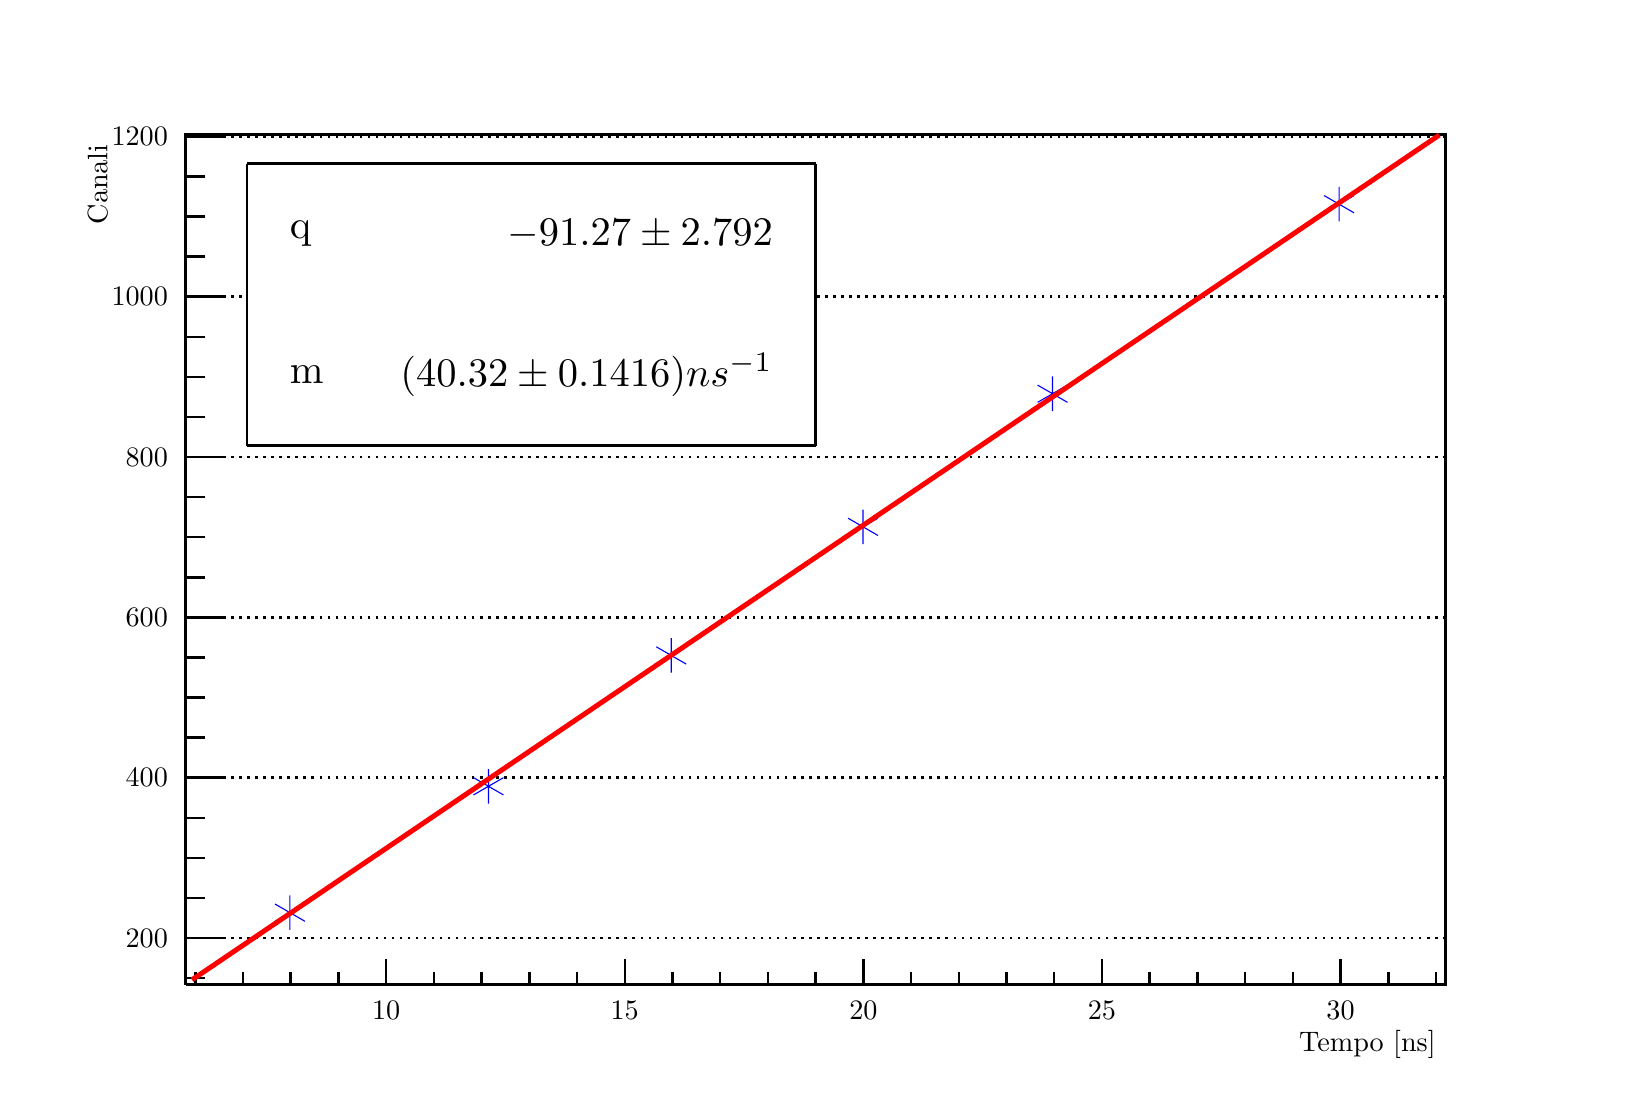
\begin{tikzpicture}
\pgfdeclareplotmark{cross} {
\pgfpathmoveto{\pgfpoint{-0.3\pgfplotmarksize}{\pgfplotmarksize}}
\pgfpathlineto{\pgfpoint{+0.3\pgfplotmarksize}{\pgfplotmarksize}}
\pgfpathlineto{\pgfpoint{+0.3\pgfplotmarksize}{0.3\pgfplotmarksize}}
\pgfpathlineto{\pgfpoint{+1\pgfplotmarksize}{0.3\pgfplotmarksize}}
\pgfpathlineto{\pgfpoint{+1\pgfplotmarksize}{-0.3\pgfplotmarksize}}
\pgfpathlineto{\pgfpoint{+0.3\pgfplotmarksize}{-0.3\pgfplotmarksize}}
\pgfpathlineto{\pgfpoint{+0.3\pgfplotmarksize}{-1.\pgfplotmarksize}}
\pgfpathlineto{\pgfpoint{-0.3\pgfplotmarksize}{-1.\pgfplotmarksize}}
\pgfpathlineto{\pgfpoint{-0.3\pgfplotmarksize}{-0.3\pgfplotmarksize}}
\pgfpathlineto{\pgfpoint{-1.\pgfplotmarksize}{-0.3\pgfplotmarksize}}
\pgfpathlineto{\pgfpoint{-1.\pgfplotmarksize}{0.3\pgfplotmarksize}}
\pgfpathlineto{\pgfpoint{-0.3\pgfplotmarksize}{0.3\pgfplotmarksize}}
\pgfpathclose
\pgfusepathqstroke
}
\pgfdeclareplotmark{cross*} {
\pgfpathmoveto{\pgfpoint{-0.3\pgfplotmarksize}{\pgfplotmarksize}}
\pgfpathlineto{\pgfpoint{+0.3\pgfplotmarksize}{\pgfplotmarksize}}
\pgfpathlineto{\pgfpoint{+0.3\pgfplotmarksize}{0.3\pgfplotmarksize}}
\pgfpathlineto{\pgfpoint{+1\pgfplotmarksize}{0.3\pgfplotmarksize}}
\pgfpathlineto{\pgfpoint{+1\pgfplotmarksize}{-0.3\pgfplotmarksize}}
\pgfpathlineto{\pgfpoint{+0.3\pgfplotmarksize}{-0.3\pgfplotmarksize}}
\pgfpathlineto{\pgfpoint{+0.3\pgfplotmarksize}{-1.\pgfplotmarksize}}
\pgfpathlineto{\pgfpoint{-0.3\pgfplotmarksize}{-1.\pgfplotmarksize}}
\pgfpathlineto{\pgfpoint{-0.3\pgfplotmarksize}{-0.3\pgfplotmarksize}}
\pgfpathlineto{\pgfpoint{-1.\pgfplotmarksize}{-0.3\pgfplotmarksize}}
\pgfpathlineto{\pgfpoint{-1.\pgfplotmarksize}{0.3\pgfplotmarksize}}
\pgfpathlineto{\pgfpoint{-0.3\pgfplotmarksize}{0.3\pgfplotmarksize}}
\pgfpathclose
\pgfusepathqfillstroke
}
\pgfdeclareplotmark{newstar} {
\pgfpathmoveto{\pgfqpoint{0pt}{\pgfplotmarksize}}
\pgfpathlineto{\pgfqpointpolar{44}{0.5\pgfplotmarksize}}
\pgfpathlineto{\pgfqpointpolar{18}{\pgfplotmarksize}}
\pgfpathlineto{\pgfqpointpolar{-20}{0.5\pgfplotmarksize}}
\pgfpathlineto{\pgfqpointpolar{-54}{\pgfplotmarksize}}
\pgfpathlineto{\pgfqpointpolar{-90}{0.5\pgfplotmarksize}}
\pgfpathlineto{\pgfqpointpolar{234}{\pgfplotmarksize}}
\pgfpathlineto{\pgfqpointpolar{198}{0.5\pgfplotmarksize}}
\pgfpathlineto{\pgfqpointpolar{162}{\pgfplotmarksize}}
\pgfpathlineto{\pgfqpointpolar{134}{0.5\pgfplotmarksize}}
\pgfpathclose
\pgfusepathqstroke
}
\pgfdeclareplotmark{newstar*} {
\pgfpathmoveto{\pgfqpoint{0pt}{\pgfplotmarksize}}
\pgfpathlineto{\pgfqpointpolar{44}{0.5\pgfplotmarksize}}
\pgfpathlineto{\pgfqpointpolar{18}{\pgfplotmarksize}}
\pgfpathlineto{\pgfqpointpolar{-20}{0.5\pgfplotmarksize}}
\pgfpathlineto{\pgfqpointpolar{-54}{\pgfplotmarksize}}
\pgfpathlineto{\pgfqpointpolar{-90}{0.5\pgfplotmarksize}}
\pgfpathlineto{\pgfqpointpolar{234}{\pgfplotmarksize}}
\pgfpathlineto{\pgfqpointpolar{198}{0.5\pgfplotmarksize}}
\pgfpathlineto{\pgfqpointpolar{162}{\pgfplotmarksize}}
\pgfpathlineto{\pgfqpointpolar{134}{0.5\pgfplotmarksize}}
\pgfpathclose
\pgfusepathqfillstroke
}
\definecolor{c}{rgb}{1,1,1};
\draw [color=c, fill=c] (0,0) rectangle (20,13.4957);
\draw [color=c, fill=c] (2,1.34957) rectangle (18,12.1461);
\definecolor{c}{rgb}{0,0,0};
\draw [c,line width=0.9] (2,1.34957) -- (2,12.1461) -- (18,12.1461) -- (18,1.34957) -- (2,1.34957);
\definecolor{c}{rgb}{1,1,1};
\draw [color=c, fill=c] (2,1.34957) rectangle (18,12.1461);
\definecolor{c}{rgb}{0,0,0};
\draw [c,line width=0.9] (2,1.34957) -- (2,12.1461) -- (18,12.1461) -- (18,1.34957) -- (2,1.34957);
\draw [c,line width=0.9] (2,1.34957) -- (18,1.34957);
\draw [c,line width=0.9] (2,1.34957) -- (2,12.1461);
\draw [c,dotted,line width=0.9] (18,1.94079) -- (2,1.94079);
\draw [c,dotted,line width=0.9] (18,3.97703) -- (2,3.97703);
\draw [c,dotted,line width=0.9] (18,6.01328) -- (2,6.01328);
\draw [c,dotted,line width=0.9] (18,8.04952) -- (2,8.04952);
\draw [c,dotted,line width=0.9] (18,10.0858) -- (2,10.0858);
\draw [c,dotted,line width=0.9] (18,12.122) -- (2,12.122);
\draw [c,dotted,line width=0.9] (18,1.94079) -- (2,1.94079);
\draw [c,dotted,line width=0.9] (18,12.122) -- (2,12.122);
\draw [c,line width=0.9] (2,1.34957) -- (18,1.34957);
\draw [anchor= east] (18,0.593811) node[scale=1.01821, color=c, rotate=0]{Tempo [ns]};
\draw [c,line width=0.9] (4.54545,1.67347) -- (4.54545,1.34957);
\draw [c,line width=0.9] (5.15152,1.51152) -- (5.15152,1.34957);
\draw [c,line width=0.9] (5.75758,1.51152) -- (5.75758,1.34957);
\draw [c,line width=0.9] (6.36364,1.51152) -- (6.36364,1.34957);
\draw [c,line width=0.9] (6.9697,1.51152) -- (6.9697,1.34957);
\draw [c,line width=0.9] (7.57576,1.67347) -- (7.57576,1.34957);
\draw [c,line width=0.9] (8.18182,1.51152) -- (8.18182,1.34957);
\draw [c,line width=0.9] (8.78788,1.51152) -- (8.78788,1.34957);
\draw [c,line width=0.9] (9.39394,1.51152) -- (9.39394,1.34957);
\draw [c,line width=0.9] (10,1.51152) -- (10,1.34957);
\draw [c,line width=0.9] (10.6061,1.67347) -- (10.6061,1.34957);
\draw [c,line width=0.9] (11.2121,1.51152) -- (11.2121,1.34957);
\draw [c,line width=0.9] (11.8182,1.51152) -- (11.8182,1.34957);
\draw [c,line width=0.9] (12.4242,1.51152) -- (12.4242,1.34957);
\draw [c,line width=0.9] (13.0303,1.51152) -- (13.0303,1.34957);
\draw [c,line width=0.9] (13.6364,1.67347) -- (13.6364,1.34957);
\draw [c,line width=0.9] (14.2424,1.51152) -- (14.2424,1.34957);
\draw [c,line width=0.9] (14.8485,1.51152) -- (14.8485,1.34957);
\draw [c,line width=0.9] (15.4545,1.51152) -- (15.4545,1.34957);
\draw [c,line width=0.9] (16.0606,1.51152) -- (16.0606,1.34957);
\draw [c,line width=0.9] (16.6667,1.67347) -- (16.6667,1.34957);
\draw [c,line width=0.9] (4.54545,1.67347) -- (4.54545,1.34957);
\draw [c,line width=0.9] (3.93939,1.51152) -- (3.93939,1.34957);
\draw [c,line width=0.9] (3.33333,1.51152) -- (3.33333,1.34957);
\draw [c,line width=0.9] (2.72727,1.51152) -- (2.72727,1.34957);
\draw [c,line width=0.9] (2.12121,1.51152) -- (2.12121,1.34957);
\draw [c,line width=0.9] (16.6667,1.67347) -- (16.6667,1.34957);
\draw [c,line width=0.9] (17.2727,1.51152) -- (17.2727,1.34957);
\draw [c,line width=0.9] (17.8788,1.51152) -- (17.8788,1.34957);
\draw [anchor=base] (4.54545,0.904212) node[scale=1.01821, color=c, rotate=0]{10};
\draw [anchor=base] (7.57576,0.904212) node[scale=1.01821, color=c, rotate=0]{15};
\draw [anchor=base] (10.6061,0.904212) node[scale=1.01821, color=c, rotate=0]{20};
\draw [anchor=base] (13.6364,0.904212) node[scale=1.01821, color=c, rotate=0]{25};
\draw [anchor=base] (16.6667,0.904212) node[scale=1.01821, color=c, rotate=0]{30};
\draw [c,line width=0.9] (2,1.34957) -- (2,12.1461);
\draw [anchor= east] (0.88,12.1461) node[scale=1.01821, color=c, rotate=90]{Canali};
\draw [c,line width=0.9] (2.48,1.94079) -- (2,1.94079);
\draw [c,line width=0.9] (2.24,2.44985) -- (2,2.44985);
\draw [c,line width=0.9] (2.24,2.95891) -- (2,2.95891);
\draw [c,line width=0.9] (2.24,3.46797) -- (2,3.46797);
\draw [c,line width=0.9] (2.48,3.97703) -- (2,3.97703);
\draw [c,line width=0.9] (2.24,4.4861) -- (2,4.4861);
\draw [c,line width=0.9] (2.24,4.99516) -- (2,4.99516);
\draw [c,line width=0.9] (2.24,5.50422) -- (2,5.50422);
\draw [c,line width=0.9] (2.48,6.01328) -- (2,6.01328);
\draw [c,line width=0.9] (2.24,6.52234) -- (2,6.52234);
\draw [c,line width=0.9] (2.24,7.0314) -- (2,7.0314);
\draw [c,line width=0.9] (2.24,7.54046) -- (2,7.54046);
\draw [c,line width=0.9] (2.48,8.04952) -- (2,8.04952);
\draw [c,line width=0.9] (2.24,8.55858) -- (2,8.55858);
\draw [c,line width=0.9] (2.24,9.06764) -- (2,9.06764);
\draw [c,line width=0.9] (2.24,9.5767) -- (2,9.5767);
\draw [c,line width=0.9] (2.48,10.0858) -- (2,10.0858);
\draw [c,line width=0.9] (2.24,10.5948) -- (2,10.5948);
\draw [c,line width=0.9] (2.24,11.1039) -- (2,11.1039);
\draw [c,line width=0.9] (2.24,11.6129) -- (2,11.6129);
\draw [c,line width=0.9] (2.48,12.122) -- (2,12.122);
\draw [c,line width=0.9] (2.48,1.94079) -- (2,1.94079);
\draw [c,line width=0.9] (2.24,1.43173) -- (2,1.43173);
\draw [c,line width=0.9] (2.48,12.122) -- (2,12.122);
\draw [anchor= east] (1.9,1.94079) node[scale=1.01821, color=c, rotate=0]{200};
\draw [anchor= east] (1.9,3.97703) node[scale=1.01821, color=c, rotate=0]{400};
\draw [anchor= east] (1.9,6.01328) node[scale=1.01821, color=c, rotate=0]{600};
\draw [anchor= east] (1.9,8.04952) node[scale=1.01821, color=c, rotate=0]{800};
\draw [anchor= east] (1.9,10.0858) node[scale=1.01821, color=c, rotate=0]{1000};
\draw [anchor= east] (1.9,12.122) node[scale=1.01821, color=c, rotate=0]{1200};
\definecolor{c}{rgb}{1,1,1};
\draw [color=c, fill=c] (2.77937,8.19484) rectangle (10,11.7765);
\definecolor{c}{rgb}{0,0,0};
\draw [c,line width=0.9] (2.77937,8.19484) -- (10,8.19484);
\draw [c,line width=0.9] (10,8.19484) -- (10,11.7765);
\draw [c,line width=0.9] (10,11.7765) -- (2.77937,11.7765);
\draw [c,line width=0.9] (2.77937,11.7765) -- (2.77937,8.19484);
\draw [anchor= west] (3.1404,10.8811) node[scale=1.46368, color=c, rotate=0]{q      };
\draw [anchor= east] (9.63897,10.8811) node[scale=1.46368, color=c, rotate=0]{$ -91.27 \pm 2.792$};
\draw [anchor= west] (3.1404,9.09026) node[scale=1.46368, color=c, rotate=0]{m       };
\draw [anchor= east] (9.63897,9.09026) node[scale=1.46368, color=c, rotate=0]{$ 40.32 \pm 0.1416$};
\definecolor{c}{rgb}{0,0,1};
\foreach \P in {(3.32378,2.26361),(5.84527,3.86819),(8.16619,5.53009),(10.6017,7.16332),(13.0086,8.85387),(16.6476,11.2607)}{\draw[mark options={color=c,fill=c},mark size=6.246246pt,mark=asterisk] plot coordinates {\P};}
\definecolor{c}{rgb}{1,0,0};
\draw [c,line width=1.8] (2.08,1.41032) -- (2.24,1.51869) -- (2.4,1.62706) -- (2.56,1.73543) -- (2.72,1.8438) -- (2.88,1.95217) -- (3.04,2.06054) -- (3.2,2.16891) -- (3.36,2.27728) -- (3.52,2.38564) -- (3.68,2.49401) -- (3.84,2.60238) -- (4,2.71075)
 -- (4.16,2.81912) -- (4.32,2.92749) -- (4.48,3.03586) -- (4.64,3.14423) -- (4.8,3.2526) -- (4.96,3.36097) -- (5.12,3.46934) -- (5.28,3.57771) -- (5.44,3.68608) -- (5.6,3.79445) -- (5.76,3.90282) -- (5.92,4.01119) -- (6.08,4.11956) -- (6.24,4.22793)
 -- (6.4,4.3363) -- (6.56,4.44467) -- (6.72,4.55303) -- (6.88,4.6614) -- (7.04,4.76977) -- (7.2,4.87814) -- (7.36,4.98651) -- (7.52,5.09488) -- (7.68,5.20325) -- (7.84,5.31162) -- (8,5.41999) -- (8.16,5.52836) -- (8.32,5.63673) -- (8.48,5.7451) --
 (8.64,5.85347) -- (8.8,5.96184) -- (8.96,6.07021) -- (9.12,6.17858) -- (9.28,6.28695) -- (9.44,6.39532) -- (9.6,6.50369) -- (9.76,6.61206) -- (9.92,6.72042);
\draw [c,line width=1.8] (9.92,6.72042) -- (10.08,6.82879) -- (10.24,6.93716) -- (10.4,7.04553) -- (10.56,7.1539) -- (10.72,7.26227) -- (10.88,7.37064) -- (11.04,7.47901) -- (11.2,7.58738) -- (11.36,7.69575) -- (11.52,7.80412) -- (11.68,7.91249) --
 (11.84,8.02086) -- (12,8.12923) -- (12.16,8.2376) -- (12.32,8.34597) -- (12.48,8.45434) -- (12.64,8.56271) -- (12.8,8.67108) -- (12.96,8.77944) -- (13.12,8.88781) -- (13.28,8.99618) -- (13.44,9.10455) -- (13.6,9.21292) -- (13.76,9.32129) --
 (13.92,9.42966) -- (14.08,9.53803) -- (14.24,9.6464) -- (14.4,9.75477) -- (14.56,9.86314) -- (14.72,9.97151) -- (14.88,10.0799) -- (15.04,10.1882) -- (15.2,10.2966) -- (15.36,10.405) -- (15.52,10.5134) -- (15.68,10.6217) -- (15.84,10.7301) --
 (16,10.8385) -- (16.16,10.9468) -- (16.32,11.0552) -- (16.48,11.1636) -- (16.64,11.2719) -- (16.8,11.3803) -- (16.96,11.4887) -- (17.12,11.5971) -- (17.28,11.7054) -- (17.44,11.8138) -- (17.6,11.9222) -- (17.76,12.0305);
\draw [c,line width=1.8] (17.76,12.0305) -- (17.92,12.1389);
\definecolor{c}{rgb}{1,1,1};
\draw [color=c, fill=c] (2.77937,8.19484) rectangle (10,11.7765);
\definecolor{c}{rgb}{0,0,0};
\draw [c,line width=0.9] (2.77937,8.19484) -- (10,8.19484);
\draw [c,line width=0.9] (10,8.19484) -- (10,11.7765);
\draw [c,line width=0.9] (10,11.7765) -- (2.77937,11.7765);
\draw [c,line width=0.9] (2.77937,11.7765) -- (2.77937,8.19484);
\draw [anchor= west] (3.1404,10.8811) node[scale=1.46368, color=c, rotate=0]{q       };
\draw [anchor= east] (9.63897,10.8811) node[scale=1.46368, color=c, rotate=0]{$ -91.27 \pm 2.792$};
\draw [anchor= west] (3.1404,9.09026) node[scale=1.46368, color=c, rotate=0]{m       };
\draw [anchor= east] (9.63897,9.09026) node[scale=1.46368, color=c, rotate=0]{$ (40.32 \pm 0.1416) ns^{-1}$};
%\draw (10.3438,12.6648) node[scale=1.40004, color=c, rotate=0]{Tempo vs Canali};
\end{tikzpicture}

%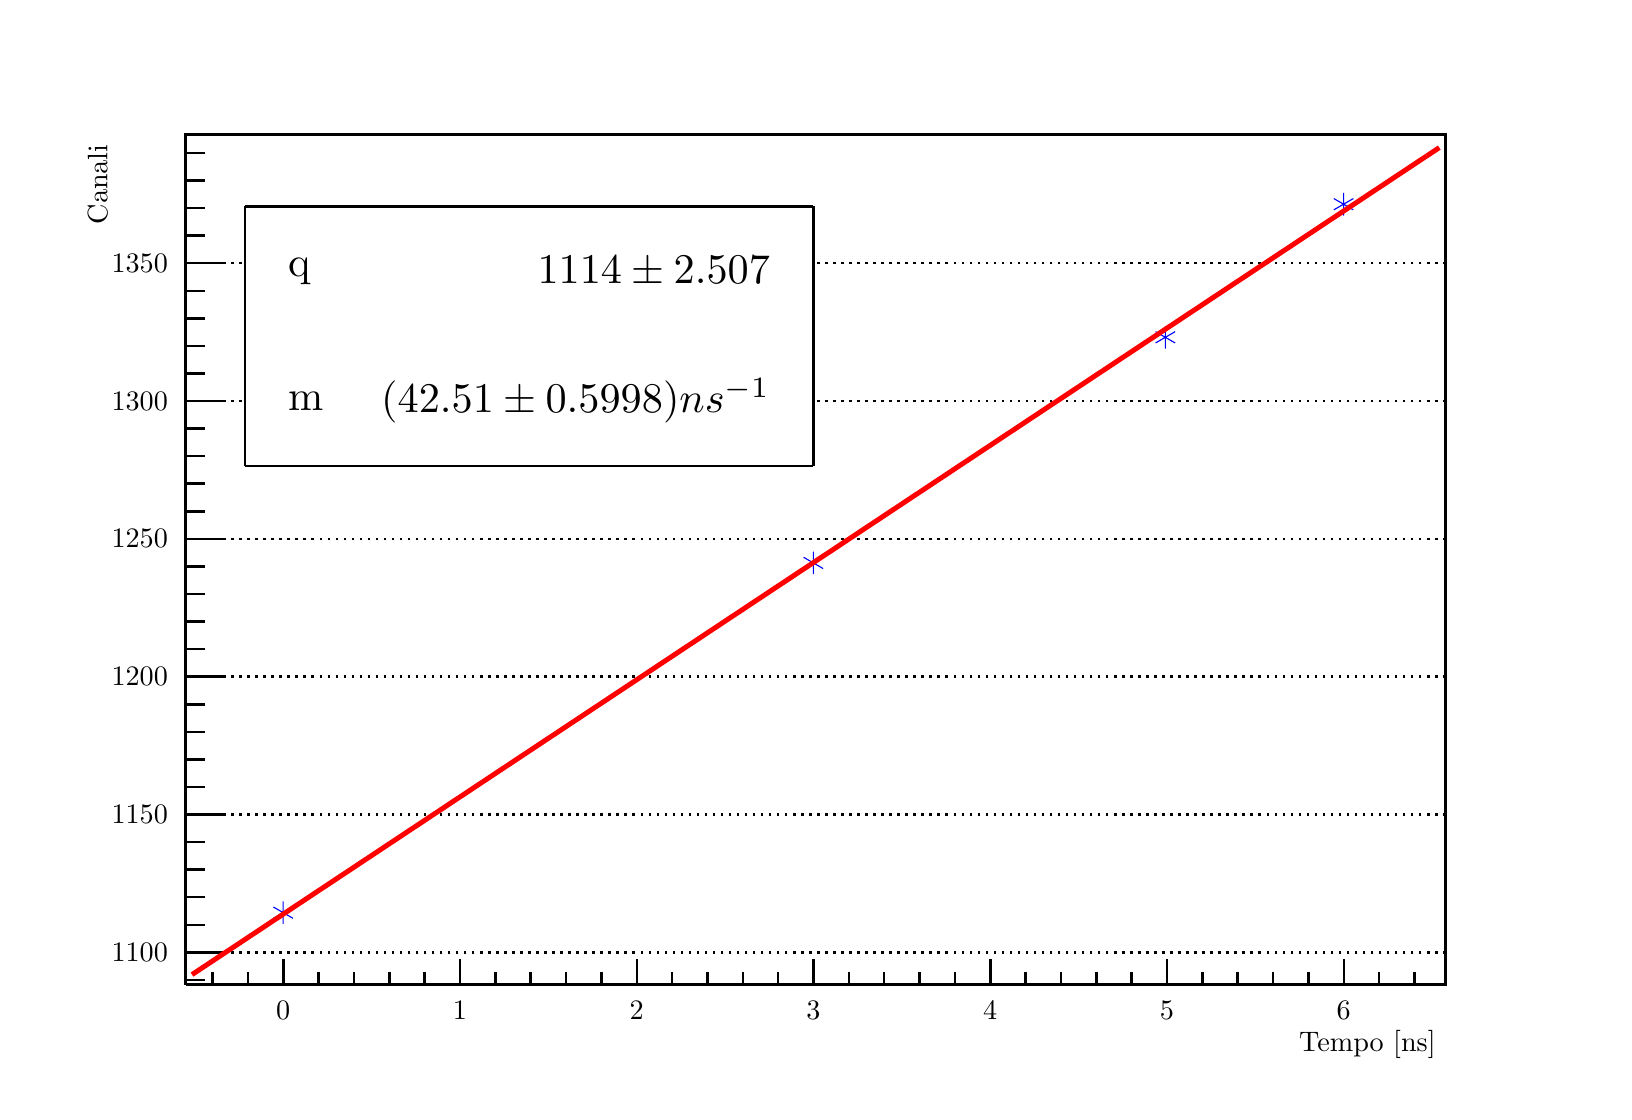
\begin{tikzpicture}
\pgfdeclareplotmark{cross} {
\pgfpathmoveto{\pgfpoint{-0.3\pgfplotmarksize}{\pgfplotmarksize}}
\pgfpathlineto{\pgfpoint{+0.3\pgfplotmarksize}{\pgfplotmarksize}}
\pgfpathlineto{\pgfpoint{+0.3\pgfplotmarksize}{0.3\pgfplotmarksize}}
\pgfpathlineto{\pgfpoint{+1\pgfplotmarksize}{0.3\pgfplotmarksize}}
\pgfpathlineto{\pgfpoint{+1\pgfplotmarksize}{-0.3\pgfplotmarksize}}
\pgfpathlineto{\pgfpoint{+0.3\pgfplotmarksize}{-0.3\pgfplotmarksize}}
\pgfpathlineto{\pgfpoint{+0.3\pgfplotmarksize}{-1.\pgfplotmarksize}}
\pgfpathlineto{\pgfpoint{-0.3\pgfplotmarksize}{-1.\pgfplotmarksize}}
\pgfpathlineto{\pgfpoint{-0.3\pgfplotmarksize}{-0.3\pgfplotmarksize}}
\pgfpathlineto{\pgfpoint{-1.\pgfplotmarksize}{-0.3\pgfplotmarksize}}
\pgfpathlineto{\pgfpoint{-1.\pgfplotmarksize}{0.3\pgfplotmarksize}}
\pgfpathlineto{\pgfpoint{-0.3\pgfplotmarksize}{0.3\pgfplotmarksize}}
\pgfpathclose
\pgfusepathqstroke
}
\pgfdeclareplotmark{cross*} {
\pgfpathmoveto{\pgfpoint{-0.3\pgfplotmarksize}{\pgfplotmarksize}}
\pgfpathlineto{\pgfpoint{+0.3\pgfplotmarksize}{\pgfplotmarksize}}
\pgfpathlineto{\pgfpoint{+0.3\pgfplotmarksize}{0.3\pgfplotmarksize}}
\pgfpathlineto{\pgfpoint{+1\pgfplotmarksize}{0.3\pgfplotmarksize}}
\pgfpathlineto{\pgfpoint{+1\pgfplotmarksize}{-0.3\pgfplotmarksize}}
\pgfpathlineto{\pgfpoint{+0.3\pgfplotmarksize}{-0.3\pgfplotmarksize}}
\pgfpathlineto{\pgfpoint{+0.3\pgfplotmarksize}{-1.\pgfplotmarksize}}
\pgfpathlineto{\pgfpoint{-0.3\pgfplotmarksize}{-1.\pgfplotmarksize}}
\pgfpathlineto{\pgfpoint{-0.3\pgfplotmarksize}{-0.3\pgfplotmarksize}}
\pgfpathlineto{\pgfpoint{-1.\pgfplotmarksize}{-0.3\pgfplotmarksize}}
\pgfpathlineto{\pgfpoint{-1.\pgfplotmarksize}{0.3\pgfplotmarksize}}
\pgfpathlineto{\pgfpoint{-0.3\pgfplotmarksize}{0.3\pgfplotmarksize}}
\pgfpathclose
\pgfusepathqfillstroke
}
\pgfdeclareplotmark{newstar} {
\pgfpathmoveto{\pgfqpoint{0pt}{\pgfplotmarksize}}
\pgfpathlineto{\pgfqpointpolar{44}{0.5\pgfplotmarksize}}
\pgfpathlineto{\pgfqpointpolar{18}{\pgfplotmarksize}}
\pgfpathlineto{\pgfqpointpolar{-20}{0.5\pgfplotmarksize}}
\pgfpathlineto{\pgfqpointpolar{-54}{\pgfplotmarksize}}
\pgfpathlineto{\pgfqpointpolar{-90}{0.5\pgfplotmarksize}}
\pgfpathlineto{\pgfqpointpolar{234}{\pgfplotmarksize}}
\pgfpathlineto{\pgfqpointpolar{198}{0.5\pgfplotmarksize}}
\pgfpathlineto{\pgfqpointpolar{162}{\pgfplotmarksize}}
\pgfpathlineto{\pgfqpointpolar{134}{0.5\pgfplotmarksize}}
\pgfpathclose
\pgfusepathqstroke
}
\pgfdeclareplotmark{newstar*} {
\pgfpathmoveto{\pgfqpoint{0pt}{\pgfplotmarksize}}
\pgfpathlineto{\pgfqpointpolar{44}{0.5\pgfplotmarksize}}
\pgfpathlineto{\pgfqpointpolar{18}{\pgfplotmarksize}}
\pgfpathlineto{\pgfqpointpolar{-20}{0.5\pgfplotmarksize}}
\pgfpathlineto{\pgfqpointpolar{-54}{\pgfplotmarksize}}
\pgfpathlineto{\pgfqpointpolar{-90}{0.5\pgfplotmarksize}}
\pgfpathlineto{\pgfqpointpolar{234}{\pgfplotmarksize}}
\pgfpathlineto{\pgfqpointpolar{198}{0.5\pgfplotmarksize}}
\pgfpathlineto{\pgfqpointpolar{162}{\pgfplotmarksize}}
\pgfpathlineto{\pgfqpointpolar{134}{0.5\pgfplotmarksize}}
\pgfpathclose
\pgfusepathqfillstroke
}
\definecolor{c}{rgb}{1,1,1};
\draw [color=c, fill=c] (0,0) rectangle (20,13.4957);
\draw [color=c, fill=c] (2,1.34957) rectangle (18,12.1461);
\definecolor{c}{rgb}{0,0,0};
\draw [c,line width=0.9] (2,1.34957) -- (2,12.1461) -- (18,12.1461) -- (18,1.34957) -- (2,1.34957);
\definecolor{c}{rgb}{1,1,1};
\draw [color=c, fill=c] (2,1.34957) rectangle (18,12.1461);
\definecolor{c}{rgb}{0,0,0};
\draw [c,line width=0.9] (2,1.34957) -- (2,12.1461) -- (18,12.1461) -- (18,1.34957) -- (2,1.34957);
\draw [c,line width=0.9] (2,1.34957) -- (18,1.34957);
\draw [c,line width=0.9] (2,1.34957) -- (2,12.1461);
\draw [c,dotted,line width=0.9] (18,1.75917) -- (2,1.75917);
\draw [c,dotted,line width=0.9] (18,3.50958) -- (2,3.50958);
\draw [c,dotted,line width=0.9] (18,5.26) -- (2,5.26);
\draw [c,dotted,line width=0.9] (18,7.01041) -- (2,7.01041);
\draw [c,dotted,line width=0.9] (18,8.76083) -- (2,8.76083);
\draw [c,dotted,line width=0.9] (18,10.5112) -- (2,10.5112);
\draw [c,dotted,line width=0.9] (18,1.75917) -- (2,1.75917);
\draw [c,dotted,line width=0.9] (18,10.5112) -- (2,10.5112);
\draw [c,line width=0.9] (2,1.34957) -- (18,1.34957);
\draw [anchor= east] (18,0.593811) node[scale=1.01821, color=c, rotate=0]{Tempo [ns]};
\draw [c,line width=0.9] (3.23906,1.67347) -- (3.23906,1.34957);
\draw [c,line width=0.9] (3.68799,1.51152) -- (3.68799,1.34957);
\draw [c,line width=0.9] (4.13692,1.51152) -- (4.13692,1.34957);
\draw [c,line width=0.9] (4.58586,1.51152) -- (4.58586,1.34957);
\draw [c,line width=0.9] (5.03479,1.51152) -- (5.03479,1.34957);
\draw [c,line width=0.9] (5.48373,1.67347) -- (5.48373,1.34957);
\draw [c,line width=0.9] (5.93266,1.51152) -- (5.93266,1.34957);
\draw [c,line width=0.9] (6.38159,1.51152) -- (6.38159,1.34957);
\draw [c,line width=0.9] (6.83053,1.51152) -- (6.83053,1.34957);
\draw [c,line width=0.9] (7.27946,1.51152) -- (7.27946,1.34957);
\draw [c,line width=0.9] (7.72839,1.67347) -- (7.72839,1.34957);
\draw [c,line width=0.9] (8.17733,1.51152) -- (8.17733,1.34957);
\draw [c,line width=0.9] (8.62626,1.51152) -- (8.62626,1.34957);
\draw [c,line width=0.9] (9.0752,1.51152) -- (9.0752,1.34957);
\draw [c,line width=0.9] (9.52413,1.51152) -- (9.52413,1.34957);
\draw [c,line width=0.9] (9.97306,1.67347) -- (9.97306,1.34957);
\draw [c,line width=0.9] (10.422,1.51152) -- (10.422,1.34957);
\draw [c,line width=0.9] (10.8709,1.51152) -- (10.8709,1.34957);
\draw [c,line width=0.9] (11.3199,1.51152) -- (11.3199,1.34957);
\draw [c,line width=0.9] (11.7688,1.51152) -- (11.7688,1.34957);
\draw [c,line width=0.9] (12.2177,1.67347) -- (12.2177,1.34957);
\draw [c,line width=0.9] (12.6667,1.51152) -- (12.6667,1.34957);
\draw [c,line width=0.9] (13.1156,1.51152) -- (13.1156,1.34957);
\draw [c,line width=0.9] (13.5645,1.51152) -- (13.5645,1.34957);
\draw [c,line width=0.9] (14.0135,1.51152) -- (14.0135,1.34957);
\draw [c,line width=0.9] (14.4624,1.67347) -- (14.4624,1.34957);
\draw [c,line width=0.9] (14.9113,1.51152) -- (14.9113,1.34957);
\draw [c,line width=0.9] (15.3603,1.51152) -- (15.3603,1.34957);
\draw [c,line width=0.9] (15.8092,1.51152) -- (15.8092,1.34957);
\draw [c,line width=0.9] (16.2581,1.51152) -- (16.2581,1.34957);
\draw [c,line width=0.9] (16.7071,1.67347) -- (16.7071,1.34957);
\draw [c,line width=0.9] (3.23906,1.67347) -- (3.23906,1.34957);
\draw [c,line width=0.9] (2.79012,1.51152) -- (2.79012,1.34957);
\draw [c,line width=0.9] (2.34119,1.51152) -- (2.34119,1.34957);
\draw [c,line width=0.9] (16.7071,1.67347) -- (16.7071,1.34957);
\draw [c,line width=0.9] (17.156,1.51152) -- (17.156,1.34957);
\draw [c,line width=0.9] (17.6049,1.51152) -- (17.6049,1.34957);
\draw [anchor=base] (3.23906,0.904212) node[scale=1.01821, color=c, rotate=0]{0};
\draw [anchor=base] (5.48373,0.904212) node[scale=1.01821, color=c, rotate=0]{1};
\draw [anchor=base] (7.72839,0.904212) node[scale=1.01821, color=c, rotate=0]{2};
\draw [anchor=base] (9.97306,0.904212) node[scale=1.01821, color=c, rotate=0]{3};
\draw [anchor=base] (12.2177,0.904212) node[scale=1.01821, color=c, rotate=0]{4};
\draw [anchor=base] (14.4624,0.904212) node[scale=1.01821, color=c, rotate=0]{5};
\draw [anchor=base] (16.7071,0.904212) node[scale=1.01821, color=c, rotate=0]{6};
\draw [c,line width=0.9] (2,1.34957) -- (2,12.1461);
\draw [anchor= east] (0.88,12.1461) node[scale=1.01821, color=c, rotate=90]{Canali};
\draw [c,line width=0.9] (2.48,1.75917) -- (2,1.75917);
\draw [c,line width=0.9] (2.24,2.10925) -- (2,2.10925);
\draw [c,line width=0.9] (2.24,2.45933) -- (2,2.45933);
\draw [c,line width=0.9] (2.24,2.80942) -- (2,2.80942);
\draw [c,line width=0.9] (2.24,3.1595) -- (2,3.1595);
\draw [c,line width=0.9] (2.48,3.50958) -- (2,3.50958);
\draw [c,line width=0.9] (2.24,3.85967) -- (2,3.85967);
\draw [c,line width=0.9] (2.24,4.20975) -- (2,4.20975);
\draw [c,line width=0.9] (2.24,4.55983) -- (2,4.55983);
\draw [c,line width=0.9] (2.24,4.90991) -- (2,4.90991);
\draw [c,line width=0.9] (2.48,5.26) -- (2,5.26);
\draw [c,line width=0.9] (2.24,5.61008) -- (2,5.61008);
\draw [c,line width=0.9] (2.24,5.96016) -- (2,5.96016);
\draw [c,line width=0.9] (2.24,6.31025) -- (2,6.31025);
\draw [c,line width=0.9] (2.24,6.66033) -- (2,6.66033);
\draw [c,line width=0.9] (2.48,7.01041) -- (2,7.01041);
\draw [c,line width=0.9] (2.24,7.3605) -- (2,7.3605);
\draw [c,line width=0.9] (2.24,7.71058) -- (2,7.71058);
\draw [c,line width=0.9] (2.24,8.06066) -- (2,8.06066);
\draw [c,line width=0.9] (2.24,8.41075) -- (2,8.41075);
\draw [c,line width=0.9] (2.48,8.76083) -- (2,8.76083);
\draw [c,line width=0.9] (2.24,9.11091) -- (2,9.11091);
\draw [c,line width=0.9] (2.24,9.46099) -- (2,9.46099);
\draw [c,line width=0.9] (2.24,9.81108) -- (2,9.81108);
\draw [c,line width=0.9] (2.24,10.1612) -- (2,10.1612);
\draw [c,line width=0.9] (2.48,10.5112) -- (2,10.5112);
\draw [c,line width=0.9] (2.48,1.75917) -- (2,1.75917);
\draw [c,line width=0.9] (2.24,1.40908) -- (2,1.40908);
\draw [c,line width=0.9] (2.48,10.5112) -- (2,10.5112);
\draw [c,line width=0.9] (2.24,10.8613) -- (2,10.8613);
\draw [c,line width=0.9] (2.24,11.2114) -- (2,11.2114);
\draw [c,line width=0.9] (2.24,11.5615) -- (2,11.5615);
\draw [c,line width=0.9] (2.24,11.9116) -- (2,11.9116);
\draw [anchor= east] (1.9,1.75917) node[scale=1.01821, color=c, rotate=0]{1100};
\draw [anchor= east] (1.9,3.50958) node[scale=1.01821, color=c, rotate=0]{1150};
\draw [anchor= east] (1.9,5.26) node[scale=1.01821, color=c, rotate=0]{1200};
\draw [anchor= east] (1.9,7.01041) node[scale=1.01821, color=c, rotate=0]{1250};
\draw [anchor= east] (1.9,8.76083) node[scale=1.01821, color=c, rotate=0]{1300};
\draw [anchor= east] (1.9,10.5112) node[scale=1.01821, color=c, rotate=0]{1350};
\definecolor{c}{rgb}{1,1,1};
\draw [color=c, fill=c] (2.75072,7.93696) rectangle (9.97135,11.2321);
\definecolor{c}{rgb}{0,0,0};
\draw [c,line width=0.9] (2.75072,7.93696) -- (9.97135,7.93696);
\draw [c,line width=0.9] (9.97135,7.93696) -- (9.97135,11.2321);
\draw [c,line width=0.9] (9.97135,11.2321) -- (2.75072,11.2321);
\draw [c,line width=0.9] (2.75072,11.2321) -- (2.75072,7.93696);
\draw [anchor= west] (3.11175,10.4083) node[scale=1.52731, color=c, rotate=0]{q       };
\draw [anchor= east] (9.61032,10.4083) node[scale=1.52731, color=c, rotate=0]{$  1114 \pm 2.507$};
\draw [anchor= west] (3.11175,8.76075) node[scale=1.52731, color=c, rotate=0]{m       };
\draw [anchor= east] (9.61032,8.76075) node[scale=1.52731, color=c, rotate=0]{$ 42.51 \pm 0.5998$};
\definecolor{c}{rgb}{0,0,1};
\foreach \P in {(3.23782,2.26361),(9.97135,6.70487),(14.4413,9.5702),(16.7049,11.2607)}{\draw[mark options={color=c,fill=c},mark size=4.084084pt,mark=asterisk] plot coordinates {\P};}
\definecolor{c}{rgb}{1,0,0};
\draw [c,line width=1.8] (2.08,1.47669) -- (2.24,1.58277) -- (2.4,1.68886) -- (2.56,1.79494) -- (2.72,1.90103) -- (2.88,2.00711) -- (3.04,2.1132) -- (3.2,2.21929) -- (3.36,2.32537) -- (3.52,2.43146) -- (3.68,2.53754) -- (3.84,2.64363) -- (4,2.74971)
 -- (4.16,2.8558) -- (4.32,2.96189) -- (4.48,3.06797) -- (4.64,3.17406) -- (4.8,3.28014) -- (4.96,3.38623) -- (5.12,3.49231) -- (5.28,3.5984) -- (5.44,3.70448) -- (5.6,3.81057) -- (5.76,3.91666) -- (5.92,4.02274) -- (6.08,4.12883) -- (6.24,4.23491)
 -- (6.4,4.341) -- (6.56,4.44708) -- (6.72,4.55317) -- (6.88,4.65926) -- (7.04,4.76534) -- (7.2,4.87143) -- (7.36,4.97751) -- (7.52,5.0836) -- (7.68,5.18968) -- (7.84,5.29577) -- (8,5.40186) -- (8.16,5.50794) -- (8.32,5.61403) -- (8.48,5.72011) --
 (8.64,5.8262) -- (8.8,5.93228) -- (8.96,6.03837) -- (9.12,6.14446) -- (9.28,6.25054) -- (9.44,6.35663) -- (9.6,6.46271) -- (9.76,6.5688) -- (9.92,6.67488);
\draw [c,line width=1.8] (9.92,6.67488) -- (10.08,6.78097) -- (10.24,6.88706) -- (10.4,6.99314) -- (10.56,7.09923) -- (10.72,7.20531) -- (10.88,7.3114) -- (11.04,7.41748) -- (11.2,7.52357) -- (11.36,7.62965) -- (11.52,7.73574) -- (11.68,7.84183) --
 (11.84,7.94791) -- (12,8.054) -- (12.16,8.16008) -- (12.32,8.26617) -- (12.48,8.37226) -- (12.64,8.47834) -- (12.8,8.58443) -- (12.96,8.69051) -- (13.12,8.7966) -- (13.28,8.90268) -- (13.44,9.00877) -- (13.6,9.11485) -- (13.76,9.22094) --
 (13.92,9.32703) -- (14.08,9.43311) -- (14.24,9.5392) -- (14.4,9.64528) -- (14.56,9.75137) -- (14.72,9.85745) -- (14.88,9.96354) -- (15.04,10.0696) -- (15.2,10.1757) -- (15.36,10.2818) -- (15.52,10.3879) -- (15.68,10.494) -- (15.84,10.6001) --
 (16,10.7061) -- (16.16,10.8122) -- (16.32,10.9183) -- (16.48,11.0244) -- (16.64,11.1305) -- (16.8,11.2366) -- (16.96,11.3427) -- (17.12,11.4487) -- (17.28,11.5548) -- (17.44,11.6609) -- (17.6,11.767) -- (17.76,11.8731);
\draw [c,line width=1.8] (17.76,11.8731) -- (17.92,11.9792);
\definecolor{c}{rgb}{1,1,1};
\draw [color=c, fill=c] (2.75072,7.93696) rectangle (9.97135,11.2321);
\definecolor{c}{rgb}{0,0,0};
\draw [c,line width=0.9] (2.75072,7.93696) -- (9.97135,7.93696);
\draw [c,line width=0.9] (9.97135,7.93696) -- (9.97135,11.2321);
\draw [c,line width=0.9] (9.97135,11.2321) -- (2.75072,11.2321);
\draw [c,line width=0.9] (2.75072,11.2321) -- (2.75072,7.93696);
\draw [anchor= west] (3.11175,10.4083) node[scale=1.52731, color=c, rotate=0]{q       };
\draw [anchor= east] (9.61032,10.4083) node[scale=1.52731, color=c, rotate=0]{$  1114 \pm 2.507$};
\draw [anchor= west] (3.11175,8.76075) node[scale=1.52731, color=c, rotate=0]{m       };
\draw [anchor= east] (9.61032,8.76075) node[scale=1.52731, color=c, rotate=0]{$ (42.51 \pm 0.5998) ns^{-1}$};
%\draw (9.55587,12.808) node[scale=1.40004, color=c, rotate=0]{Calibrazione Cavi};
\end{tikzpicture}


La dipendenza lineare attesa è stata ben riscontrata.
A seguito di tale calibrazione è stato possibile ricavare il ritardo associato all'inserimento di cavi LEMO tra il Delay e lo stop del TAC ricavando il centroide dai vari spettri del 
TAC ed associandovi un ritardo ricavato tramite i parametri del precedente fit. La relazione lineare che vede in ascissa i tempi ed i relativi centroidi in ordinata è stata 
quindi invertita ricavandosi per propagazione gli errori sui nuovi parametri ed ottenendo i seguenti risultati. Il ritardo associato ai cavetti di diversa lunghezza è molto simile
a quello indicato, la differenza è forse dovuta ad approssimazioni o ad effetti strumentali.\\

\begin{tabella}[h]
	\centering
	\begin{center}
\begin{tabulary}{\textwidth}{CCCCC}
\toprule
Cavo	& Centroide	& Sigma centroide	& Tempo	[ns]	& Sigma tempo [ns]	\\ \midrule
3 ns	& 1241		& 0.1 			& 3.0		& 0.1			\\ \midrule
5 ns	& 1323		& 0.2 			& 5.1		& 0.1			\\ \midrule
6 ns	& 1371		& 0.2 			& 6.3 		& 0.1			\\
\bottomrule
\end{tabulary}
\end{center}

	\caption{Stima del ritardo introdotto dai cavi}
	\label{tab:calib_cavi}
\end{tabella}
 
Infine si è verificato che il delay esterno del CFD che massimizzasse la risoluzione fosse quello di 4ns, ottenuto tramite un apposito cavo LEMO. Si sono confrontati tre diversi cavi
che determinassero un ritardo da 3ns, 4ns e 5ns acquisendo lo spettro del TAC e limitandosi a confrontare solamene le sigma essendo i centroidi sostanzialmente uguali. Ciò che si 
è osservato è che il picco con sigma minore era quello relatvo al ritardo da 4ns, determinando quindi la scelta di usare tale cavo per le misure succesive. Di seguito in tabella
i risultati dei fit gaussiani in canali effettuati sugli spettri\footnote{Come prima, nelle appendici si possono vedere i grafici delle interpolazioni gaussiane.}. \\

\begin{tabella}[h]
	\centering
	\begin{center}
\begin{tabulary}{\textwidth}{CCCCC}
\toprule
Cavi	& Centroide 	& Errore Centroide 	& Sigma 	& Errore sigma	\\ \midrule
 3 ns	&	1270	&	0.1		&	11.29	&	0.01	\\ \midrule
 4 ns	&	1263	&	0.1		&	11.11	&	0.03	\\ \midrule
 5 ns	&	1269	&	0.1		&	13.09	&	0.02	\\
\bottomrule
\end{tabulary}
\end{center}

	\caption{Stima del ritardo introdotto dai cavi}
	\label{tab:calib_cavi}
\end{tabella}



